\documentclass[11pt,letterpaper]{article}

\usepackage[margin=1in]{geometry}
\usepackage{amsmath,amssymb}
\usepackage{listings}
\usepackage{xcolor}
\usepackage{hyperref}
\usepackage{booktabs}
\usepackage{graphicx}
\usepackage{tikz}
\usetikzlibrary{arrows.meta, positioning, shapes.geometric, fit, calc, decorations.pathreplacing}
\usepackage{caption}
\usepackage{subcaption}
\usepackage{microtype}
\usepackage{parskip}
\usepackage{enumitem}
\usepackage{fancyhdr}
\usepackage{titlesec}
\usepackage{array}
\usepackage{multirow}

% Code listing style
\lstdefinestyle{cpp}{
  language=C++,
  basicstyle=\ttfamily\small,
  keywordstyle=\color{blue}\bfseries,
  commentstyle=\color{gray}\itshape,
  stringstyle=\color{red!70!black},
  numbers=left,
  numberstyle=\tiny\color{gray},
  numbersep=8pt,
  breaklines=true,
  frame=single,
  rulecolor=\color{black!20},
  backgroundcolor=\color{gray!5},
  tabsize=2,
  showstringspaces=false,
  captionpos=b,
}

\lstdefinestyle{bash}{
  language=bash,
  basicstyle=\ttfamily\small,
  keywordstyle=\color{teal}\bfseries,
  commentstyle=\color{gray}\itshape,
  numbers=none,
  frame=single,
  rulecolor=\color{black!20},
  backgroundcolor=\color{gray!5},
  breaklines=true,
  showstringspaces=false,
}

\hypersetup{
  colorlinks=true,
  linkcolor=blue!70!black,
  urlcolor=blue!70!black,
  citecolor=green!50!black,
}

\pagestyle{fancy}
\fancyhf{}
\rhead{NEXUS Multi-GPU FHE --- Code Study}
\lhead{Comp 390 --- Spring 2026}
\cfoot{\thepage}

\title{\textbf{NEXUS \& Phantom FHE: A Complete Code Study}\\
\large GPU-Accelerated Fully Homomorphic Encryption for Multi-GPU Extension}
\author{Halil Ibrahim Kanpak \\ Comp 390 Independent Study, Spring 2026}
\date{March 2026}

\begin{document}
\maketitle

%------------------------------------------------------------
\begin{abstract}
This document explains the NEXUS GPU-accelerated Fully Homomorphic Encryption (FHE) inference
system from the ground up. NEXUS (Zhang et al., NDSS 2025) is the first system to run a full
BERT-base transformer entirely on encrypted data, achieving 37 seconds per inference on a
single NVIDIA A100. It is built on top of Phantom, a GPU-native library implementing the CKKS
FHE scheme. Our project extends NEXUS from one GPU to many GPUs (and eventually many nodes) by
distributing the RNS limbs --- the modular components of each ciphertext --- across GPUs using
NCCL collective operations. This document covers the cryptographic foundations, the Phantom
library data structures, the NEXUS neural-network operations, our multi-GPU design, a
performance model, and a profiling guide. It is written for a reader new to both CUDA
and FHE.
\end{abstract}

\tableofcontents
\newpage

%============================================================
\section{Introduction}
%============================================================

\subsection{Why Privacy-Preserving Inference?}

Machine learning inference usually requires sending plaintext data to a server. This creates
a privacy problem: a hospital querying an AI diagnostic model must expose patient records to
the server operator. Fully Homomorphic Encryption solves this by allowing the server to
compute on \emph{encrypted} data --- the server never sees the underlying patient data, and
only the client (who holds the secret key) can read the result.

Until recently, FHE was too slow for real neural networks. NEXUS changed that: by using the
CKKS scheme on NVIDIA A100 GPUs, it runs BERT-base inference in 37 seconds on a single GPU.
The remaining bottleneck is that BERT-base has 12 layers, each requiring expensive
cryptographic operations. Running inference faster requires more GPUs.

\subsection{The Parallelism Opportunity}

The key insight is that CKKS represents each encrypted value as a polynomial whose coefficients
are split across many \emph{RNS limbs} --- independent arrays of 64-bit integers. Each limb is
mathematically independent from the others for most operations (NTT, addition, plaintext
multiplication). This makes limbs the natural unit of parallelism: GPU $g$ takes ownership of
limbs $j$ where $j \bmod n_\text{GPUs} = g$, and each GPU works on its own slice with no
communication required for those operations.

The one operation that does require communication is \emph{key-switching} (used for
relinearization after multiplication, and for rotation). Key-switching requires contributions
from all limbs. We implement and compare two algorithms for distributing it across GPUs using
NCCL collectives.

\subsection{How to Read This Document}

The document builds from foundations to implementation:
\begin{enumerate}[noitemsep]
  \item \textbf{Section~\ref{sec:background}}: FHE math --- CKKS, RNS, NTT, key-switching, bootstrapping.
  \item \textbf{Section~\ref{sec:structure}}: Repository layout.
  \item \textbf{Sections~\ref{sec:phantom-data}--\ref{sec:phantom-ops}}: Phantom library internals.
  \item \textbf{Sections~\ref{sec:nexus-eval}--\ref{sec:nexus-ops}}: NEXUS neural network operations.
  \item \textbf{Section~\ref{sec:perfmodel}}: Analytical performance model for multi-GPU.
  \item \textbf{Sections~\ref{sec:multigpu}--\ref{sec:srcfiles}}: Our multi-GPU design and code.
  \item \textbf{Sections~\ref{sec:build}--\ref{sec:profiling}}: Build instructions and profiling guide.
\end{enumerate}

%============================================================
\section{Background: Fully Homomorphic Encryption}
\label{sec:background}
%============================================================

\subsection{What Is FHE?}

Fully Homomorphic Encryption (FHE) allows arbitrary computations to be performed on
\emph{encrypted} data without ever decrypting it. The data owner encrypts their input, sends
the ciphertext to a server, the server computes on the ciphertext, and returns an encrypted
result. Only the data owner, who holds the secret key, can decrypt the final answer.

This is powerful for privacy-preserving machine learning: a hospital could encrypt patient
data, send it to an AI inference server, and receive encrypted diagnoses --- with the server
never seeing the actual patient data.

\subsection{The CKKS Scheme}

NEXUS uses the \textbf{CKKS} (Cheon-Kim-Kim-Song) FHE scheme, designed specifically for
real-number arithmetic. Key properties:

\begin{itemize}
  \item \textbf{Plaintext space:} A vector of up to $N/2$ complex (or real) floating-point numbers, where $N$ is the polynomial degree.
  \item \textbf{Approximate arithmetic:} Results are approximate, with a controllable error. This is acceptable for neural network inference.
  \item \textbf{SIMD packing:} All $N/2$ slots are processed in \emph{one} FHE operation (Single Instruction, Multiple Data). NEXUS uses $N = 65536$, giving $32768$ slots per ciphertext.
  \item \textbf{Scaling factor:} Real numbers are scaled up to integers (e.g., by $2^{40}$) before encryption. Each multiplication doubles the scale, requiring a ``rescale'' step to bring it back.
\end{itemize}

\subsection{Ring Learning With Errors (RLWE)}

The security of CKKS rests on the Ring Learning With Errors (RLWE) problem. A ciphertext is
a pair of polynomials $(c_0, c_1)$ in the ring $\mathbb{Z}_Q[x]/(x^N + 1)$:

\[
c_0 = a \cdot s + e + m, \quad c_1 = -a
\]

where $s$ is the secret key polynomial, $a$ is a uniformly random polynomial, $e$ is a small
noise polynomial, and $m$ encodes the plaintext message. Given only $(c_0, c_1)$, recovering
$m$ requires solving RLWE, which is believed to be computationally hard.

\subsection{Residue Number System (RNS) Representation}

The modulus $Q$ in CKKS is a 512--2000 bit integer, far too large to store as a single machine
word. Instead, CKKS decomposes $Q$ as a product of small primes:
\[
Q = q_0 \cdot q_1 \cdot q_2 \cdots q_{L-1}
\]

Each prime $q_i$ fits in a 64-bit integer. By the Chinese Remainder Theorem (CRT), arithmetic
modulo $Q$ can be performed independently modulo each small prime, then recombined. Each
prime's contribution is called an \textbf{RNS limb}.

\textbf{Key implication for multi-GPU:} Each RNS limb is an independent array of $N$
64-bit integers. Limbs can be distributed across GPUs --- GPU $g$ computes limbs $i$ where
$i \bmod n\_\text{GPUs} = g$.

\subsection{Number Theoretic Transform (NTT)}

The Number Theoretic Transform (NTT) is the modular-arithmetic analogue of the Fast Fourier
Transform (FFT). It converts a polynomial from \emph{coefficient form} (list of coefficients
$a_0, a_1, \ldots, a_{N-1}$) to \emph{evaluation form} (values at $N$ special roots of
unity), and back. NTT form enables polynomial multiplication to be done via pointwise
multiplication instead of convolution --- reducing complexity from $O(N^2)$ to $O(N \log N)$.

All ciphertexts in NEXUS are stored in NTT form on the GPU. The Phantom library uses a
\textbf{2D radix-8 NTT kernel} optimized for NVIDIA GPUs.

\subsection{The Modulus Chain and Levels}
\label{sec:modchain}

Each FHE multiplication consumes one ``level'': it requires a \textbf{rescale} step that
divides the ciphertext by one prime and drops it from the chain. Starting with $L$ primes
(level 0), after one multiply+rescale we have $L-1$ primes (level 1), and so on. When only
one prime remains, no more multiplications are possible.

Figure~\ref{fig:modchain} shows this consumption process for the GELU benchmark ($L=20$).

\begin{figure}[h]
\centering
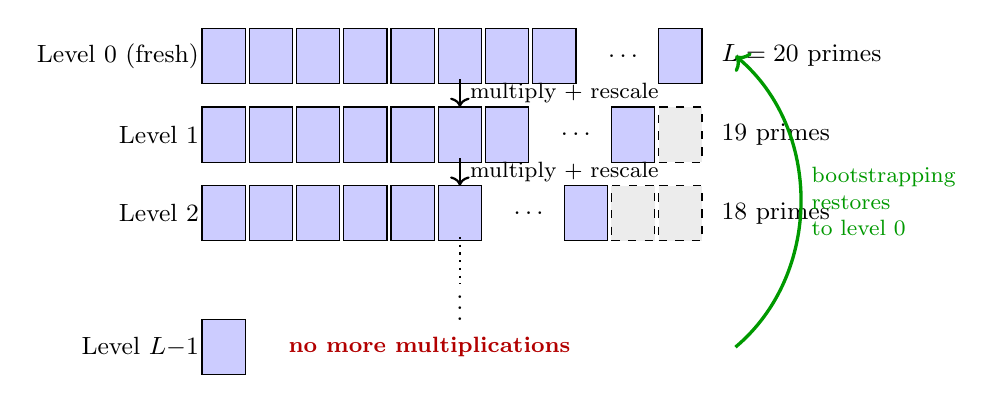
\begin{tikzpicture}[
  prime/.style={draw, fill=blue!20, minimum width=0.55cm, minimum height=0.7cm, font=\tiny},
  dropped/.style={draw, fill=gray!15, minimum width=0.55cm, minimum height=0.7cm, font=\tiny, dashed},
  every node/.style={font=\small}
]
  % Level 0: all 20 primes (shown condensed)
  \node[anchor=east] at (-0.1, 2) {Level 0 (fresh):};
  \foreach \i in {0,...,7} {
    \node[prime] at (\i*0.6, 2) {};
  }
  \node at (5.1, 2) {\ldots};
  \node[prime] at (5.8, 2) {};
  \node[right] at (6.2, 2) {$L=20$ primes};

  % Arrow down
  \draw[->, thick] (3.0, 1.7) -- (3.0, 1.35) node[midway, right, font=\footnotesize] {multiply + rescale};

  % Level 1: 19 primes
  \node[anchor=east] at (-0.1, 1) {Level 1:};
  \foreach \i in {0,...,6} {
    \node[prime] at (\i*0.6, 1) {};
  }
  \node at (4.5, 1) {\ldots};
  \node[prime] at (5.2, 1) {};
  \node[dropped] at (5.8, 1) {};
  \node[right] at (6.2, 1) {19 primes};

  % Arrow down
  \draw[->, thick] (3.0, 0.7) -- (3.0, 0.35) node[midway, right, font=\footnotesize] {multiply + rescale};

  % Level 2: 18 primes
  \node[anchor=east] at (-0.1, 0) {Level 2:};
  \foreach \i in {0,...,5} {
    \node[prime] at (\i*0.6, 0) {};
  }
  \node at (3.9, 0) {\ldots};
  \node[prime] at (4.6, 0) {};
  \node[dropped] at (5.2, 0) {};
  \node[dropped] at (5.8, 0) {};
  \node[right] at (6.2, 0) {18 primes};

  % Dotted continuation
  \draw[dotted, thick] (3.0, -0.3) -- (3.0, -0.9);
  \node at (3.0, -1.1) {$\vdots$};

  % Level L-1: 1 prime
  \node[anchor=east] at (-0.1, -1.7) {Level $L{-}1$:};
  \node[prime] at (0, -1.7) {};
  \node[right, red!70!black, font=\footnotesize\bfseries] at (0.7, -1.7) {no more multiplications};

  % Bootstrap arrow back up
  \draw[->, very thick, green!60!black, bend right=50]
    (6.5, -1.7) to node[right, green!60!black, font=\footnotesize, align=left] {bootstrapping\\restores\\to level 0}
    (6.5, 2);

\end{tikzpicture}
\caption{The modulus chain for GELU ($L=20$ primes). Each multiply+rescale drops one prime.
Bootstrapping is the expensive operation that refreshes the ciphertext back to the top level.}
\label{fig:modchain}
\end{figure}

\subsection{Key-Switching}

Key-switching is the mechanism underlying both relinearization and rotation. Given a
ciphertext's extra polynomial $c_2$ (produced during multiplication), key-switching computes
a correction that eliminates $c_2$ while maintaining the decryption invariant. It proceeds
in three stages:

\begin{enumerate}
  \item \textbf{RNS Decomposition}: $c_2$ is split into $\beta$ ``digits'' using Hybrid/HPS decomposition.
  \item \textbf{Inner Product}: Each digit is multiplied by its evaluation key component and accumulated.
  \item \textbf{Basis Extension}: The result is lifted from auxiliary basis $P$ to main basis $Q$ via CRT.
\end{enumerate}

Key-switching is the most expensive single operation in NEXUS, and it is the operation that
requires inter-GPU communication in the multi-GPU setting.

\subsection{Bootstrapping}

When a ciphertext reaches the bottom of the modulus chain (level $L-1$), it cannot be
multiplied further. Bootstrapping refreshes the ciphertext, restoring its level budget at the
cost of a large computation. The NEXUS bootstrapping pipeline uses 31 total levels (17 for
the main computation, 14 for bootstrapping itself):

\begin{enumerate}
  \item \textbf{Slot-to-Coefficient (StoC)}: Encrypted IFFT via Baby-Step Giant-Step (BSGS) --- $O(\sqrt{N})$ rotations.
  \item \textbf{Modular Reduction}: Minimax polynomial approximation of $x \bmod q$.
  \item \textbf{Coefficient-to-Slot (CtoS)}: Encrypted FFT, moving data back to slots.
\end{enumerate}

%============================================================
\section{Project Repository Structure}
\label{sec:structure}
%============================================================

\begin{lstlisting}[style=bash, caption=Top-level directory layout]
Comp390Project/
|-- vendor/
|   |-- nexus/          # NEXUS GPU inference engine (git submodule)
|   |   `-- cuda/src/   # All GPU CUDA source files
|   `-- phantom/        # Phantom FHE library (git submodule)
|-- src/
|   `-- multi_gpu/      # OUR implementation: multi-GPU extensions
|       |-- comm/        # NCCL collective wrappers
|       |-- partition/   # RNS limb-to-GPU assignment
|       |-- keyswitching/ # Multi-GPU key-switching algorithms
|       `-- overlap/     # CUDA stream management, compute/comm overlap
|-- src/benchmarks/     # Our benchmark harnesses
|-- scripts/
|   |-- aws/            # EC2 spot instance launch + env setup
|   `-- mn5/            # MareNostrum 5 SLURM scripts
|-- profiling/          # Nsight Systems / Compute scripts
|-- experiments/        # Raw results, plots, RESULTS.md index
|-- paper/              # LaTeX documents
|-- CMakeLists.txt      # Top-level build system
|-- study.md            # Literature review (36 KB)
`-- notes/log.md        # Session-by-session research log
\end{lstlisting}

%============================================================
\section{Phantom FHE Library: Data Structures}
\label{sec:phantom-data}
%============================================================

\subsection{Overview}

Phantom is a GPU-native FHE library. Unlike CPU-based libraries (Microsoft SEAL,
OpenFHE), Phantom stores all ciphertext data \emph{on the GPU} from the moment of
encryption. All arithmetic is performed on GPU memory via CUDA kernels. There is no
host--device transfer overhead during computation.

\subsection{PhantomCiphertext}

This is the central data structure. It holds two (or more) polynomials encrypted under
the CKKS scheme.

\begin{lstlisting}[style=cpp, caption=PhantomCiphertext member variables (ciphertext.h)]
class PhantomCiphertext {
private:
    phantom::parms_id_type parms_id_;   // Parameter set identifier
    size_t chain_index_ = 0;            // Level in modulus chain (0 = freshest)
    size_t size_ = 0;                   // Number of polynomials (2 = standard, 3 after multiply)
    size_t poly_modulus_degree_ = 0;    // N (ring degree, e.g. 65536)
    size_t coeff_modulus_size_ = 0;     // L = number of RNS primes at current level
    double scale_ = 1.0;               // CKKS scaling factor (e.g. 2^40)
    bool is_ntt_form_ = true;          // True if stored in NTT/evaluation form
    cuda_auto_ptr<uint64_t> data_;     // THE GPU BUFFER (all polynomial data)
};
\end{lstlisting}

\subsubsection{GPU Memory Layout}

The \texttt{data\_} buffer stores all polynomial coefficient data in a flat 3D array:

\[
\texttt{data}[\,\underbrace{i}_{\text{poly}}\;]\,[\,\underbrace{j}_{\text{limb}}\;]\,[\,\underbrace{k}_{\text{coeff}}\;]
= \texttt{data.get()} + i \cdot (N \cdot L) + j \cdot N + k
\]

\begin{itemize}
  \item $i \in \{0, 1\}$: polynomial index (fresh ciphertext has 2 polynomials: $c_0$ and $c_1$)
  \item $j \in \{0, \ldots, L-1\}$: RNS limb index (one per prime in the current modulus chain)
  \item $k \in \{0, \ldots, N-1\}$: coefficient index within one polynomial modulo one prime
\end{itemize}

Figure~\ref{fig:memlayout} shows how the flat GPU buffer maps to this 3D structure, and how
limbs are assigned to GPUs in the multi-GPU case.

\begin{figure}[h]
\centering
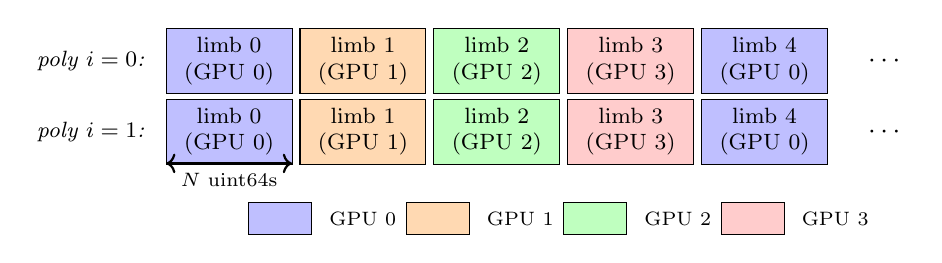
\begin{tikzpicture}[
  block/.style={draw, minimum width=1.6cm, minimum height=0.55cm, font=\footnotesize, align=center},
  gpuA/.style={block, fill=blue!25},
  gpuB/.style={block, fill=orange!30},
  gpuC/.style={block, fill=green!25},
  gpuD/.style={block, fill=red!20},
  label/.style={font=\footnotesize\itshape}
]
  % Poly 0
  \node[label, anchor=east] at (-0.1, 1.5) {poly $i=0$:};
  \node[gpuA] at (0.85,  1.5) {limb 0\\(GPU 0)};
  \node[gpuB] at (2.55,  1.5) {limb 1\\(GPU 1)};
  \node[gpuC] at (4.25,  1.5) {limb 2\\(GPU 2)};
  \node[gpuD] at (5.95,  1.5) {limb 3\\(GPU 3)};
  \node[gpuA] at (7.65,  1.5) {limb 4\\(GPU 0)};
  \node        at (9.2,   1.5) {$\cdots$};

  % Poly 1
  \node[label, anchor=east] at (-0.1, 0.6) {poly $i=1$:};
  \node[gpuA] at (0.85,  0.6) {limb 0\\(GPU 0)};
  \node[gpuB] at (2.55,  0.6) {limb 1\\(GPU 1)};
  \node[gpuC] at (4.25,  0.6) {limb 2\\(GPU 2)};
  \node[gpuD] at (5.95,  0.6) {limb 3\\(GPU 3)};
  \node[gpuA] at (7.65,  0.6) {limb 4\\(GPU 0)};
  \node        at (9.2,   0.6) {$\cdots$};

  % Annotations
  \draw[<->, thick] (0.05, 0.2) -- (1.65, 0.2)
    node[midway, below, font=\scriptsize] {$N$ uint64s};

  % Legend
  \node[gpuA, minimum width=0.8cm, minimum height=0.4cm] at (1.5, -0.5) {};
  \node[right, font=\scriptsize] at (2.0, -0.5) {GPU 0};
  \node[gpuB, minimum width=0.8cm, minimum height=0.4cm] at (3.5, -0.5) {};
  \node[right, font=\scriptsize] at (4.0, -0.5) {GPU 1};
  \node[gpuC, minimum width=0.8cm, minimum height=0.4cm] at (5.5, -0.5) {};
  \node[right, font=\scriptsize] at (6.0, -0.5) {GPU 2};
  \node[gpuD, minimum width=0.8cm, minimum height=0.4cm] at (7.5, -0.5) {};
  \node[right, font=\scriptsize] at (8.0, -0.5) {GPU 3};

\end{tikzpicture}
\caption{Ciphertext GPU memory layout. Each row is one polynomial ($c_0$ or $c_1$). Each
cell is one RNS limb: $N$ contiguous 64-bit integers. Color indicates which GPU owns each
limb under cyclic assignment ($j \bmod 4$). Every GPU holds the same number of limbs,
ensuring load balance.}
\label{fig:memlayout}
\end{figure}

\textbf{Example sizes} (GELU benchmark):
\begin{itemize}
  \item $N = 65536$, $L = 20$ RNS primes, 2 polynomials
  \item Buffer size: $2 \times 20 \times 65536 \times 8\ \text{bytes} = 20.97\ \text{MB}$ per ciphertext
\end{itemize}

The key accessor methods are:
\begin{lstlisting}[style=cpp, caption=Accessing ciphertext data pointers]
uint64_t* ct.data();           // Base pointer: poly 0, limb 0, coeff 0
uint64_t* ct.data(i);          // Pointer to start of polynomial i
// = data_.get() + i * (poly_modulus_degree_ * coeff_modulus_size_)
\end{lstlisting}

\subsection{PhantomContext and the Modulus Chain}

\texttt{PhantomContext} holds all precomputed tables and parameters for a given FHE parameter
set. The \textbf{modulus chain} is the sequence of RNS prime sets at decreasing levels:

\begin{lstlisting}[style=cpp, caption=Modulus chain for GELU benchmark (main.cu)]
// GELU uses 20 primes: 58-bit anchor + eighteen 40-bit compute primes + 58-bit tail
vector<int> gelu_moduli = {58, 40, 40, 40, 40, 40, 40, 40, 40, 40,
                            40, 40, 40, 40, 40, 40, 40, 40, 40, 58};
// Level 0 (freshest): all 20 primes active
// Level 1: 19 primes active (one dropped by rescale)
// ...
// Level 19: 1 prime active (cannot multiply further)
\end{lstlisting}

The full \texttt{PhantomContext} structure contains:
\begin{itemize}
  \item \texttt{std::vector<ContextData> context\_data\_}: One entry per chain level, each with its own RNS tools and NTT tables.
  \item \texttt{DNTTTable gpu\_rns\_tables\_}: Precomputed NTT twiddle factors for all moduli, stored on GPU.
  \item \texttt{PhantomGaloisTool* key\_galois\_tool\_}: Permutation indices for rotation operations.
\end{itemize}

\subsection{Evaluation Keys}

Three types of keys enable ciphertext operations beyond addition:

\begin{description}
  \item[\texttt{PhantomRelinKey}] Relinearization key: reduces a size-3 ciphertext (product of two size-2 ciphertexts) back to size-2. Used after every multiplication.
  \item[\texttt{PhantomGaloisKey}] Galois key set: enables rotation of the slot vector by any supported number of positions. Each rotation step $s$ needs its own Galois key.
  \item[\texttt{PhantomPublicKey}] For asymmetric encryption.
\end{description}

Keys are stored entirely on GPU memory. For $N = 65536$ and $L = 20$ primes, a single
Galois key is approximately $2 \times 20 \times 65536 \times 8\ \text{bytes} \approx 21\
\text{MB}$. NEXUS's bootstrapping uses $\sim 60$ rotation keys, totaling $\sim 1.2\ \text{GB}$
of key material on each GPU.

%============================================================
\section{Phantom FHE Library: Core Operations}
\label{sec:phantom-ops}
%============================================================

\subsection{NTT Kernels}

The Number Theoretic Transform is the computational bottleneck in almost all FHE operations.
Phantom implements a highly optimized \textbf{2D radix-8 NTT} on the GPU.

\begin{lstlisting}[style=cpp, caption=NTT kernel interface (ntt.cuh)]
// Forward NTT: coefficient form -> NTT/evaluation form (in-place)
void nwt_2d_radix8_forward_inplace(
    uint64_t *inout,              // GPU buffer: [coeff_modulus_size][poly_degree]
    const DNTTTable &ntt_tables,  // Precomputed twiddle factors
    size_t coeff_modulus_size,    // Number of RNS limbs to transform
    size_t start_modulus_idx,     // First limb index to transform
    const cudaStream_t &stream    // CUDA stream for async execution
);

// Backward NTT: NTT form -> coefficient form (in-place)
void nwt_2d_radix8_backward_inplace(/* same signature */);
\end{lstlisting}

The 2D layout means each row in the GPU grid processes one RNS limb independently --- all
$L$ limbs are transformed \emph{in parallel} on the GPU. Within each limb, the radix-8
butterfly maximizes arithmetic intensity per global memory access.

For multi-GPU, each GPU performs NTT only on its own subset of limbs. No communication is
required for NTT --- it is the only FHE operation that parallelizes perfectly.

\subsection{Key-Switching}

Given a ciphertext's extra polynomial $c_2$ (produced during multiplication), key-switching
computes a correction that eliminates $c_2$ while maintaining the decryption invariant.

\begin{lstlisting}[style=cpp, caption=Key-switching inner product kernel (evaluate.cuh)]
__global__ void key_switch_inner_prod_c2_and_evk(
    uint64_t *dst,              // Output: two new polynomials of result ciphertext
    const uint64_t *c2,         // Input: the extra polynomial to be switched
    const uint64_t *const *evks, // Evaluation keys (one per decomposition level beta)
    const DModulus *modulus,    // RNS moduli Q (current) and P (auxiliary)
    size_t n,                   // Ring degree N
    size_t size_QP,             // |Q| + |P| total moduli
    size_t size_Ql,             // |Q| at current chain level
    size_t beta,                // Number of key decomposition pieces
    ...
);
\end{lstlisting}

The algorithm proceeds in three stages:

\begin{enumerate}
  \item \textbf{RNS Decomposition}: $c_2$ is decomposed into $\beta$ ``digits'' using the
    Hybrid/HPS decomposition. Each digit is a sub-polynomial with smaller coefficient size.
  \item \textbf{Inner Product}: Each digit is multiplied by its corresponding evaluation key
    component and accumulated (inner product over $\beta$ terms).
  \item \textbf{Basis Extension}: The result, initially in the auxiliary basis $P$, is
    lifted back to the main basis $Q$ via CRT-based modular arithmetic.
\end{enumerate}

This is the operation where multi-GPU parallelism is most complex: the inner product requires
contributions from \emph{all} limbs, so GPUs must exchange partial results via NCCL AllReduce.

\subsection{CKKS Arithmetic Operations}

\begin{lstlisting}[style=cpp, caption=Core CKKS operations available in Phantom (evaluate.cuh)]
// Multiply two ciphertexts (produces size-3 result)
void multiply_inplace(PhantomCiphertext &ct1, const PhantomCiphertext &ct2, stream);

// Relinearize: reduce size 3 -> 2 using relin keys
void relinearize_inplace(PhantomCiphertext &ct, const PhantomRelinKey &rk, stream);

// Rescale: divide by one prime, dropping one level (removes scale^2 -> scale)
void rescale_to_next_inplace(PhantomCiphertext &ct, stream);

// Mod-switch: drop one prime without scaling (aligns levels between ciphertexts)
void mod_switch_to_next_inplace(PhantomCiphertext &ct, stream);

// Addition and subtraction (no level consumed)
void add_inplace(PhantomCiphertext &ct1, const PhantomCiphertext &ct2, stream);
void sub_inplace(PhantomCiphertext &ct1, const PhantomCiphertext &ct2, stream);

// Rotation: cyclic shift of slots by `steps` positions
void rotate_vector_inplace(PhantomCiphertext &ct, int steps,
                            const PhantomGaloisKey &gk, stream);

// Multiply by a plaintext constant (one level consumed after rescale)
void multiply_plain_inplace(PhantomCiphertext &ct, const PhantomPlaintext &pt, stream);
\end{lstlisting}

The computational cost hierarchy (fastest to slowest):
\begin{enumerate}
  \item Add/Sub: $O(N \cdot L)$ pointwise modular addition --- very cheap
  \item Multiply-plain: $O(N \cdot L)$ pointwise modular multiplication --- cheap
  \item NTT (forward/inverse): $O(N \cdot L \cdot \log N)$ --- moderate
  \item Multiply + Relin: $O(\beta \cdot N \cdot L)$ where $\beta \approx L/\text{digit\_size}$ --- expensive
  \item Rotation (= key-switch): Same cost as Multiply + Relin --- expensive
\end{enumerate}

%============================================================
\section{NEXUS: The CKKSEvaluator Class}
\label{sec:nexus-eval}
%============================================================

\subsection{Architecture}

NEXUS wraps Phantom in a more convenient C++ API. The central class is \texttt{CKKSEvaluator},
which bundles together all state needed for FHE inference:

\begin{lstlisting}[style=cpp, caption=CKKSEvaluator interface (ckks\_evaluator.cuh)]
class CKKSEvaluator {
public:
    PhantomContext *context;
    PhantomRelinKey *relin_keys;
    PhantomGaloisKey *galois_keys;
    vector<uint32_t> galois_elts;   // Supported rotation steps

    Encoder   encoder;    // encode/decode double vectors <-> PhantomPlaintext
    Encryptor encryptor;  // encrypt PhantomPlaintext -> PhantomCiphertext
    Evaluator evaluator;  // FHE arithmetic (delegates to Phantom)
    Decryptor decryptor;  // decrypt PhantomCiphertext -> PhantomPlaintext

    size_t degree;        // N = poly_modulus_degree
    double scale;         // CKKS scaling factor (e.g. pow(2.0, 40))
    size_t slot_count;    // N/2 real-number slots per ciphertext
};
\end{lstlisting}

\subsection{Mathematical Utility Methods}

NEXUS provides high-level FHE implementations of common mathematical functions needed for
transformer inference. Each function is a sequence of FHE operations requiring careful
management of levels and scales.

\subsubsection{Degree-9 Odd Polynomial Evaluation (\texttt{eval\_odd\_deg9\_poly})}

Evaluates $f(x) = a_9 x^9 + a_7 x^7 + a_5 x^5 + a_3 x^3 + a_1 x$ in 4
multiplications using a Paterson--Stockmeyer-like scheme:

\begin{enumerate}
  \item Compute $x^2 = x \cdot x$ (1 multiply, rescale)
  \item Compute $x^3 = x^2 \cdot x$ (1 multiply, rescale)
  \item Accumulate odd powers with careful scale management at each chain level
\end{enumerate}

This is used as a building block for approximating non-polynomial functions (GELU,
SoftMax numerics) at low multiplicative depth.

\subsubsection{Sign Function (\texttt{sgn\_eval})}

Approximates $\text{sgn}(x)$ using composite Chebyshev polynomials (minimax approximation).
The approximation alternates between two polynomial families (G and F coefficients) for $d_g$
and $d_f$ iterations respectively. Used in bootstrapping's modular reduction step.

\subsubsection{Inverse Square Root (\texttt{invert\_sqrt})}

Computes $1/\sqrt{x}$ using a combination of Newton and Goldschmidt iterations in encrypted
domain. Used in LayerNorm for normalization. The Goldschmidt iteration converges as:
\[
y_{n+1} = y_n \cdot (1.5 - 0.5 \cdot v \cdot y_n^2), \quad y_n \to 1/\sqrt{v}
\]

\subsubsection{Exponentiation (\texttt{exp})}

Computes $e^x$ via: $e^x = (1 + x/128)^{128}$. The base $(1 + x/128)$ is computed with
two FHE multiplications, and then squared $\log_2(128) = 7$ times. Total cost: 9 multiplications,
depth 9.

%============================================================
\section{NEXUS: Neural Network Operations}
\label{sec:nexus-ops}
%============================================================

\subsection{BERT-Base Architecture Overview}

BERT-base is a 12-layer Transformer encoder with hidden dimension 768, 12 attention
heads, and 110M parameters. Each layer contains:

\begin{enumerate}
  \item \textbf{Multi-Head Self-Attention (MHSA):} Three matrix multiplications (Q, K, V
    projections), attention score computation (SoftMax), and output projection.
  \item \textbf{Feed-Forward Network (FFN):} Two matrix multiplications with GELU activation
    in between.
  \item \textbf{Layer Normalization:} Applied before/after each sub-layer.
\end{enumerate}

Each of these sub-operations has a homomorphic implementation in NEXUS.
Figures~\ref{fig:toptrace} and~\ref{fig:layertrace} trace the full execution, from program
start through every encrypted operation in a single layer.

% ---------------------------------------------------------------
% Figure: Top-level execution trace (detailed, HPC-style)
% ---------------------------------------------------------------
\begin{figure}[p]
\centering
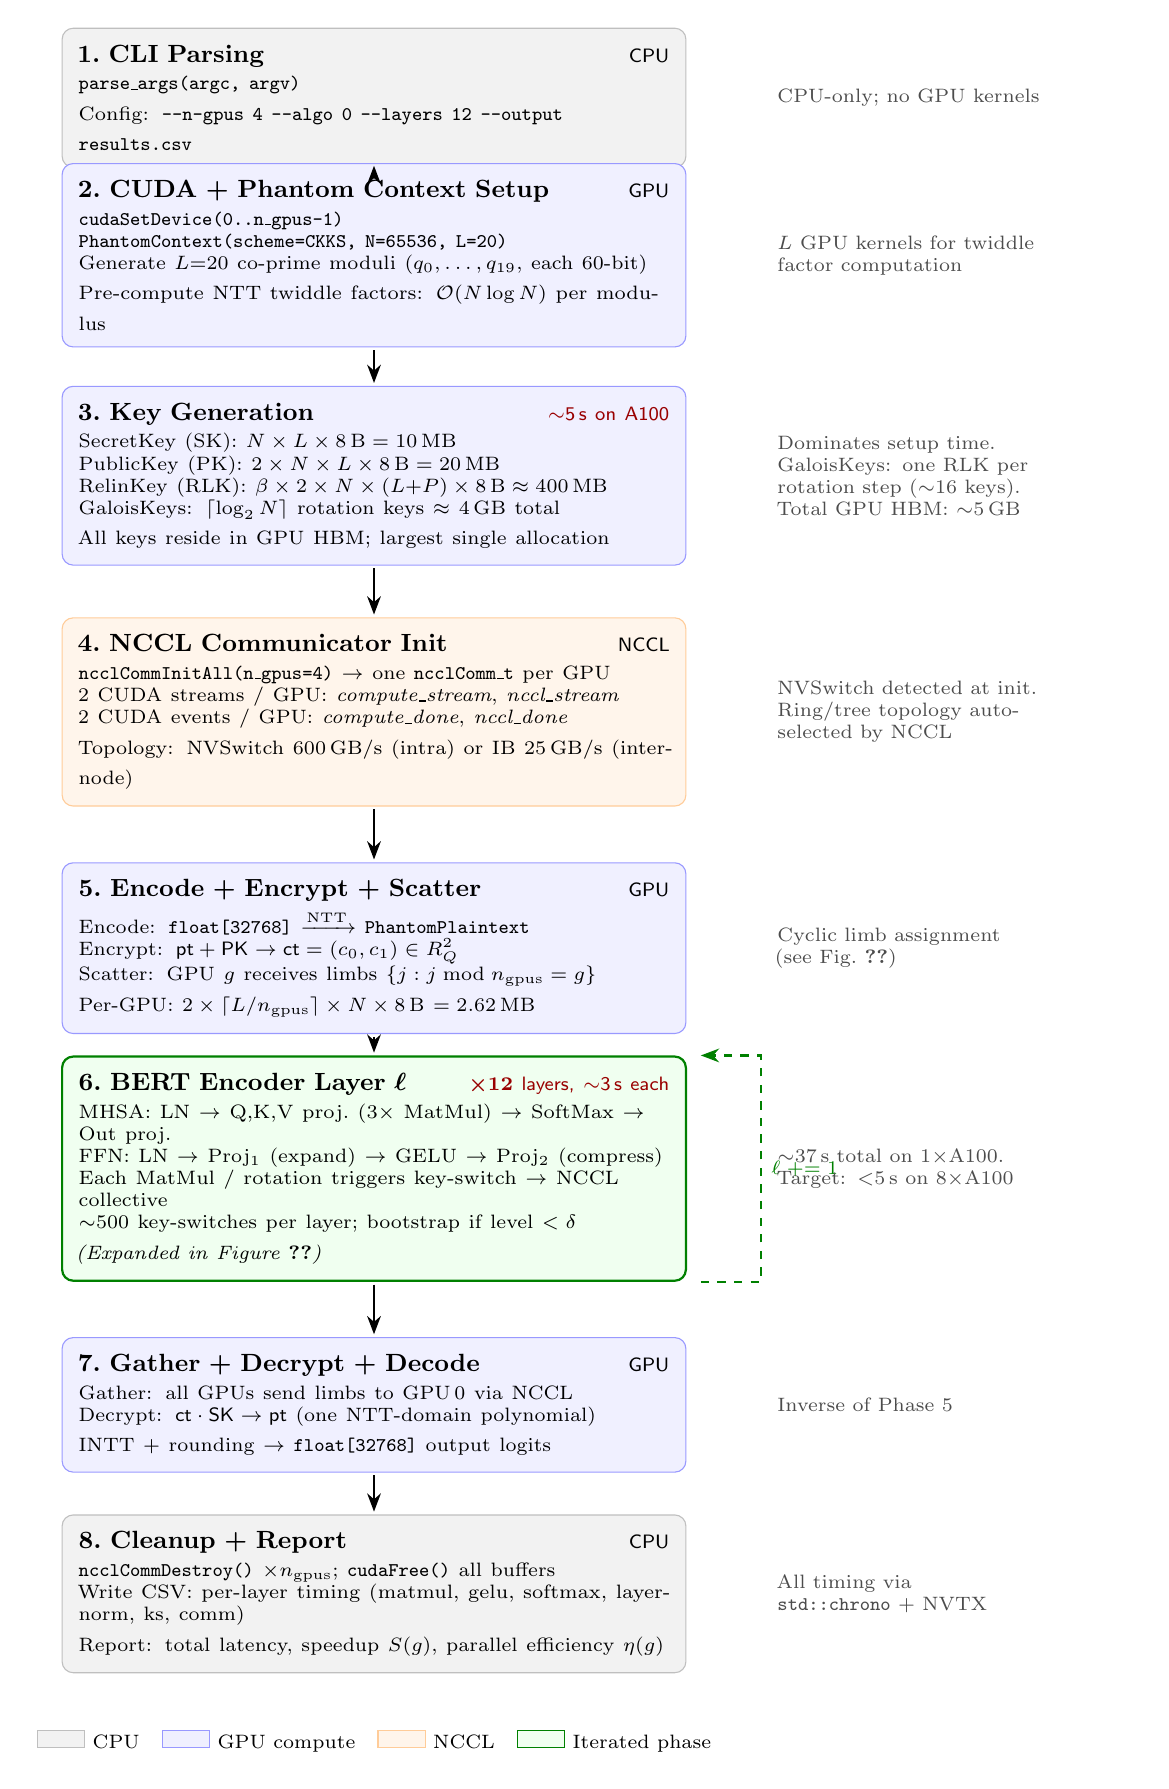
\begin{tikzpicture}[
  phase/.style={draw, rounded corners=4pt, text width=7.5cm, font=\small,
                align=left, inner sep=6pt},
  cpuph/.style={phase, fill=gray!10, draw=gray!50},
  gpuph/.style={phase, fill=blue!6, draw=blue!40},
  ncclph/.style={phase, fill=orange!8, draw=orange!40},
  loopph/.style={phase, fill=green!6, draw=green!50!black, line width=0.8pt},
  arr/.style={->, >=Stealth, thick, shorten >=1pt, shorten <=1pt},
  ann/.style={font=\scriptsize, text width=4.5cm, align=left, anchor=west,
              gray!60!black},
]

% --- Phase 1 ---
\node[cpuph] (p1) at (0, 0) {%
  \textbf{1.\ CLI Parsing} \hfill \textsf{\scriptsize CPU}\\[2pt]
  {\scriptsize\texttt{parse\_args(argc, argv)}\\
  Config: \texttt{--n-gpus 4 --algo 0 --layers 12 --output results.csv}}%
};

% --- Phase 2 ---
\node[gpuph] (p2) at (0, -2.0) {%
  \textbf{2.\ CUDA + Phantom Context Setup} \hfill \textsf{\scriptsize GPU}\\[2pt]
  {\scriptsize\texttt{cudaSetDevice(0..n\_gpus{-}1)}\\
  \texttt{PhantomContext(scheme=CKKS, N=65536, L=20)}\\
  Generate $L{=}20$ co-prime moduli ($q_0, \ldots, q_{19}$, each 60-bit)\\
  Pre-compute NTT twiddle factors: $\mathcal{O}(N \log N)$ per modulus}%
};

% --- Phase 3 ---
\node[gpuph] (p3) at (0, -4.8) {%
  \textbf{3.\ Key Generation} \hfill
    {\color{red!60!black}\textsf{\scriptsize $\sim$5\,s on A100}}\\[2pt]
  {\scriptsize%
  SecretKey (SK): $N \times L \times 8\,\text{B} = 10$\,MB\\
  PublicKey (PK): $2 \times N \times L \times 8\,\text{B} = 20$\,MB\\
  RelinKey (RLK): $\beta \times 2 \times N \times (L{+}P) \times
    8\,\text{B} \approx 400$\,MB\\
  GaloisKeys: $\lceil\log_2 N\rceil$ rotation keys $\approx$ 4\,GB
    total\\
  All keys reside in GPU HBM; largest single allocation}%
};

% --- Phase 4 ---
\node[ncclph] (p4) at (0, -7.8) {%
  \textbf{4.\ NCCL Communicator Init} \hfill \textsf{\scriptsize NCCL}\\[2pt]
  {\scriptsize%
  \texttt{ncclCommInitAll(n\_gpus=4)} $\to$ one \texttt{ncclComm\_t}
    per GPU\\
  2 CUDA streams / GPU: \textit{compute\_stream},
    \textit{nccl\_stream}\\
  2 CUDA events / GPU: \textit{compute\_done}, \textit{nccl\_done}\\
  Topology: NVSwitch 600\,GB/s (intra) or IB 25\,GB/s (inter-node)}%
};

% --- Phase 5 ---
\node[gpuph] (p5) at (0, -10.8) {%
  \textbf{5.\ Encode + Encrypt + Scatter} \hfill \textsf{\scriptsize GPU}\\[2pt]
  {\scriptsize%
  Encode: \texttt{float[32768]}
    $\xrightarrow{\text{NTT}}$ \texttt{PhantomPlaintext}\\
  Encrypt: $\mathsf{pt} + \mathsf{PK} \to \mathsf{ct} =
    (c_0, c_1) \in R_Q^2$\\
  Scatter: GPU~$g$ receives limbs
    $\{j : j \bmod n_\text{gpus} = g\}$\\
  Per-GPU: $2 \times \lceil L/n_\text{gpus}\rceil \times N \times
    8$\,B $= 2.62$\,MB}%
};

% --- Phase 6 (the loop) ---
\node[loopph] (p6) at (0, -13.6) {%
  \textbf{6.\ BERT Encoder Layer $\boldsymbol{\ell}$}
  \hfill {\color{red!60!black}\textsf{\scriptsize
    $\boldsymbol{\times 12}$ layers, $\sim$3\,s each}}\\[2pt]
  {\scriptsize%
  MHSA: LN $\to$ Q,K,V proj.\ ($3 \times$ MatMul) $\to$ SoftMax
    $\to$ Out proj.\\
  FFN: LN $\to$ Proj$_1$ (expand) $\to$ GELU $\to$ Proj$_2$
    (compress)\\
  Each MatMul / rotation triggers key-switch $\to$ NCCL collective\\
  ${\sim}$500 key-switches per layer; bootstrap if level $< \delta$\\
  \textit{(Expanded in Figure~\ref{fig:layertrace})}}%
};

% Loop-back arrow
\draw[arr, green!50!black, dashed, thick]
  ([xshift=4pt]p6.south east) -- ++(0.8, 0) |-
  ([xshift=4pt]p6.north east)
  node[pos=0.25, right, font=\scriptsize, green!50!black]
    {$\ell \mathrel{{+}{=}} 1$};

% --- Phase 7 ---
\node[gpuph] (p7) at (0, -16.6) {%
  \textbf{7.\ Gather + Decrypt + Decode} \hfill
    \textsf{\scriptsize GPU}\\[2pt]
  {\scriptsize%
  Gather: all GPUs send limbs to GPU\,0 via NCCL\\
  Decrypt: $\mathsf{ct} \cdot \mathsf{SK} \to \mathsf{pt}$
    (one NTT-domain polynomial)\\
  INTT + rounding $\to$ \texttt{float[32768]} output logits}%
};

% --- Phase 8 ---
\node[cpuph] (p8) at (0, -19.0) {%
  \textbf{8.\ Cleanup + Report} \hfill \textsf{\scriptsize CPU}\\[2pt]
  {\scriptsize%
  \texttt{ncclCommDestroy()} $\times n_\text{gpus}$;\
    \texttt{cudaFree()} all buffers\\
  Write CSV: per-layer timing (matmul, gelu, softmax, layernorm,
    ks, comm)\\
  Report: total latency, speedup $S(g)$, parallel efficiency
    $\eta(g)$}%
};

% --- Flow arrows ---
\draw[arr] (p1) -- (p2);
\draw[arr] (p2) -- (p3);
\draw[arr] (p3) -- (p4);
\draw[arr] (p4) -- (p5);
\draw[arr] (p5) -- (p6);
\draw[arr] (p6) -- (p7);
\draw[arr] (p7) -- (p8);

% --- Right-column annotations ---
\node[ann] at (5.0,  0.0)  {CPU-only; no GPU kernels};
\node[ann] at (5.0, -2.0)  {$L$ GPU kernels for twiddle\\
  factor computation};
\node[ann] at (5.0, -4.8)  {Dominates setup time.\\
  GaloisKeys: one RLK per\\
  rotation step ($\sim$16 keys).\\
  Total GPU HBM: $\sim$5\,GB};
\node[ann] at (5.0, -7.8)  {NVSwitch detected at init.\\
  Ring/tree topology auto-\\selected by NCCL};
\node[ann] at (5.0, -10.8) {Cyclic limb assignment\\
  (see Fig.~\ref{fig:memlayout})};
\node[ann] at (5.0, -13.6) {${\sim}$37\,s total on 1$\times$A100.\\
  Target: $<$5\,s on 8$\times$A100};
\node[ann] at (5.0, -16.6) {Inverse of Phase~5};
\node[ann] at (5.0, -19.0) {All timing via\\
  \texttt{std::chrono} + NVTX};

% --- Legend (single-line, bottom) ---
\node[font=\scriptsize, anchor=north] at (0, -20.6) {%
  \tikz\fill[gray!10, draw=gray!50]
    (0,0) rectangle (0.6cm,0.22cm);\ CPU\quad
  \tikz\fill[blue!6, draw=blue!40]
    (0,0) rectangle (0.6cm,0.22cm);\ GPU compute\quad
  \tikz\fill[orange!8, draw=orange!40]
    (0,0) rectangle (0.6cm,0.22cm);\ NCCL\quad
  \tikz\fill[green!6, draw=green!50!black]
    (0,0) rectangle (0.6cm,0.22cm);\ Iterated phase%
};

\end{tikzpicture}
\caption{Top-level execution trace of \texttt{bert\_inference}.
  Each box shows one program phase with exact CUDA/NCCL calls and data sizes.
  Grey$=$CPU; blue$=$GPU compute; orange$=$NCCL communication;
  green dashed$=$12-iteration inference loop (expanded in
  Figure~\ref{fig:layertrace}).
  On a single A100, key generation takes $\sim$5\,s and the 12-layer
  inference takes $\sim$37\,s total.}
\label{fig:toptrace}
\end{figure}

% ---------------------------------------------------------------
% Figure: Single BERT layer execution trace (kernel-level detail)
% ---------------------------------------------------------------
\begin{figure}[p]
\centering
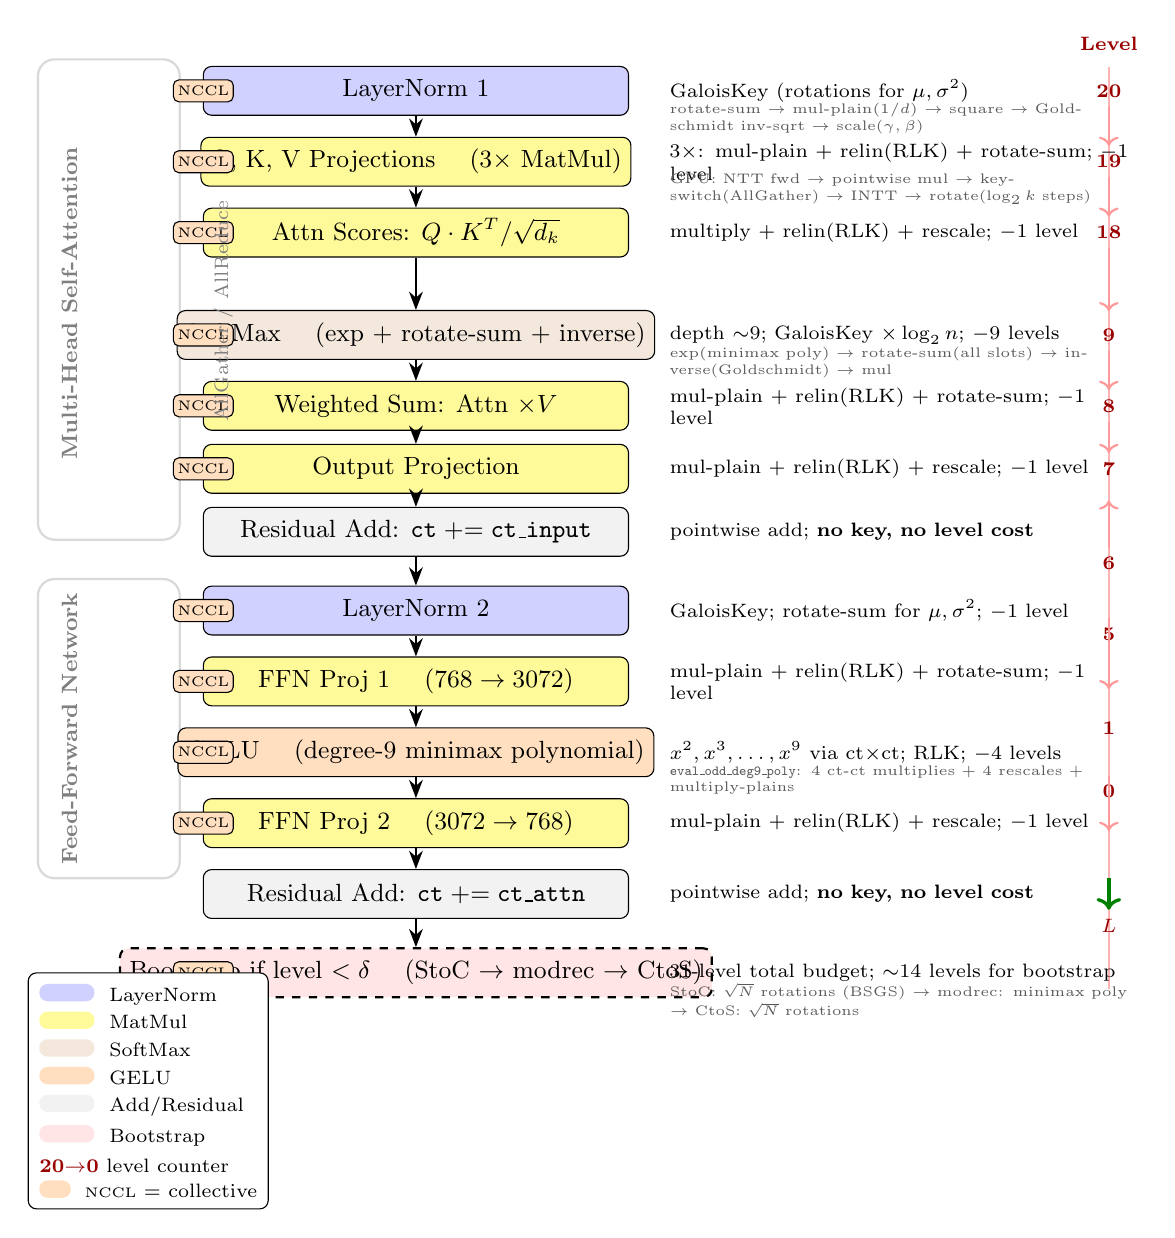
\begin{tikzpicture}[
  blk/.style={draw, rounded corners=3pt, minimum width=5.4cm,
              minimum height=0.62cm, font=\small, align=center},
  ln/.style ={blk, fill=blue!18},
  mm/.style ={blk, fill=yellow!40},
  sm/.style ={blk, fill=brown!18},
  ge/.style ={blk, fill=orange!25},
  add/.style={blk, fill=gray!10},
  boot/.style={blk, fill=red!10, dashed, line width=0.8pt},
  arr/.style={->, >=Stealth, thick},
  ann/.style={font=\scriptsize, anchor=west, align=left,
              text width=5.8cm},
  sub/.style={font=\tiny, anchor=west, align=left,
              text width=5.8cm, gray!70!black},
  ksmark/.style={draw, fill=orange!25, rounded corners=2pt,
                 font=\tiny, inner sep=1.5pt, minimum height=0.28cm},
  lvl/.style={font=\scriptsize\bfseries, red!60!black},
]
  % ===== Level counter (right edge) =====
  \node[lvl] at (8.8, 13.4) {Level};
  \draw[red!30, thick] (8.8, 13.1) -- (8.8, 1.4);
  % Level ticks (approximate for GELU context, L=20)
  \node[lvl] at (8.8, 12.8) {20};
  \node[lvl] at (8.8, 11.9) {19};
  \node[lvl] at (8.8, 11.0) {18};
  \node[lvl] at (8.8,  9.7) {9};
  \node[lvl] at (8.8,  8.8) {8};
  \node[lvl] at (8.8,  8.0) {7};
  \node[lvl] at (8.8,  6.8) {6};
  \node[lvl] at (8.8,  5.9) {5};
  \node[lvl] at (8.8,  4.7) {1};
  \node[lvl] at (8.8,  3.9) {0};
  \node[lvl] at (8.8,  2.2) {$L$};
  % Level decrease arrows
  \draw[->, red!40, thick] (8.8, 12.6) -- (8.8, 12.1);
  \draw[->, red!40, thick] (8.8, 11.7) -- (8.8, 11.2);
  \draw[->, red!40, thick] (8.8, 10.8) -- (8.8, 10.0);
  \draw[->, red!40, thick] (8.8,  9.5) -- (8.8,  9.0);
  \draw[->, red!40, thick] (8.8,  8.6) -- (8.8,  8.2);
  \draw[->, red!40, thick] (8.8,  7.0) -- (8.8,  7.6);
  \draw[->, red!40, thick] (8.8,  6.1) -- (8.8,  5.2);
  \draw[->, red!40, thick] (8.8,  4.1) -- (8.8,  3.4);
  % Bootstrap restore
  \draw[->, green!50!black, very thick] (8.8, 2.8) -- (8.8, 2.4);

  % ===== Sub-block labels =====
  \draw[gray!30, thick, rounded corners=6pt]
    (-4.8, 13.2) rectangle (-3.0, 7.1);
  \node[font=\footnotesize\bfseries, gray, rotate=90]
    at (-4.4, 10.1) {Multi-Head Self-Attention};
  \draw[gray!30, thick, rounded corners=6pt]
    (-4.8, 6.6) rectangle (-3.0, 2.8);
  \node[font=\footnotesize\bfseries, gray, rotate=90]
    at (-4.4, 4.7) {Feed-Forward Network};

  % ===== MHSA operations =====
  \node[ln]  (ln1)  at (0, 12.8) {LayerNorm 1};
  \node[mm]  (qkv)  at (0, 11.9) {Q, K, V Projections
    \quad ($3\times$ MatMul)};
  \node[mm]  (qk)   at (0, 11.0) {Attn Scores:
    $Q \cdot K^{T} / \sqrt{d_k}$};
  \node[sm]  (soft) at (0,  9.7) {SoftMax
    \quad (exp + rotate-sum + inverse)};
  \node[mm]  (av)   at (0,  8.8) {Weighted Sum:
    Attn $\times V$};
  \node[mm]  (oprj) at (0,  8.0) {Output Projection};
  \node[add] (res1) at (0,  7.2) {Residual Add:
    $\mathtt{ct} \mathrel{+}= \mathtt{ct\_input}$};

  % ===== FFN operations =====
  \node[ln]  (ln2)  at (0, 6.2) {LayerNorm 2};
  \node[mm]  (ffn1) at (0, 5.3) {FFN Proj 1
    \quad ($768 \to 3072$)};
  \node[ge]  (gelu) at (0, 4.4) {GELU
    \quad (degree-9 minimax polynomial)};
  \node[mm]  (ffn2) at (0, 3.5) {FFN Proj 2
    \quad ($3072 \to 768$)};
  \node[add] (res2) at (0, 2.6) {Residual Add:
    $\mathtt{ct} \mathrel{+}= \mathtt{ct\_attn}$};

  % ===== Bootstrap =====
  \node[boot](boot) at (0, 1.6) {Bootstrap if level
    $< \delta$ \quad (StoC $\to$ modrec $\to$ CtoS)};

  % ===== Flow arrows =====
  \draw[arr] (ln1)  -- (qkv);
  \draw[arr] (qkv)  -- (qk);
  \draw[arr] (qk)   -- (soft);
  \draw[arr] (soft) -- (av);
  \draw[arr] (av)   -- (oprj);
  \draw[arr] (oprj) -- (res1);
  \draw[arr] (res1) -- (ln2);
  \draw[arr] (ln2)  -- (ffn1);
  \draw[arr] (ffn1) -- (gelu);
  \draw[arr] (gelu) -- (ffn2);
  \draw[arr] (ffn2) -- (res2);
  \draw[arr] (res2) -- (boot);

  % ===== Right-side: key type + sub-kernel detail =====
  \node[ann] at (3.1, 12.8)
    {GaloisKey (rotations for $\mu, \sigma^2$)};
  \node[sub] at (3.1, 12.45)
    {rotate-sum $\to$ mul-plain($1/d$) $\to$ square $\to$
     Goldschmidt inv-sqrt $\to$ scale($\gamma, \beta$)};

  \node[ann] at (3.1, 11.9)
    {$3\times$: mul-plain + relin(RLK) + rotate-sum; $-1$ level};
  \node[sub] at (3.1, 11.55)
    {GPU: NTT fwd $\to$ pointwise mul $\to$ key-switch(AllGather)
     $\to$ INTT $\to$ rotate($\log_2 k$ steps)};

  \node[ann] at (3.1, 11.0)
    {multiply + relin(RLK) + rescale; $-1$ level};

  \node[ann] at (3.1, 9.7)
    {depth ${\sim}$9; GaloisKey $\times \log_2 n$; $-9$ levels};
  \node[sub] at (3.1, 9.35)
    {exp(minimax poly) $\to$ rotate-sum(all slots) $\to$
     inverse(Goldschmidt) $\to$ mul};

  \node[ann] at (3.1, 8.8)
    {mul-plain + relin(RLK) + rotate-sum; $-1$ level};

  \node[ann] at (3.1, 8.0)
    {mul-plain + relin(RLK) + rescale; $-1$ level};

  \node[ann] at (3.1, 7.2)
    {pointwise add; \textbf{no key, no level cost}};

  \node[ann] at (3.1, 6.2)
    {GaloisKey; rotate-sum for $\mu, \sigma^2$; $-1$ level};

  \node[ann] at (3.1, 5.3)
    {mul-plain + relin(RLK) + rotate-sum; $-1$ level};

  \node[ann] at (3.1, 4.4)
    {$x^2, x^3, \ldots, x^9$ via ct$\times$ct; RLK; $-4$ levels};
  \node[sub] at (3.1, 4.05)
    {\texttt{eval\_odd\_deg9\_poly}: 4 ct-ct multiplies
     + 4 rescales + multiply-plains};

  \node[ann] at (3.1, 3.5)
    {mul-plain + relin(RLK) + rescale; $-1$ level};

  \node[ann] at (3.1, 2.6)
    {pointwise add; \textbf{no key, no level cost}};

  \node[ann] at (3.1, 1.6)
    {31-level total budget; ${\sim}$14 levels for bootstrap};
  \node[sub] at (3.1, 1.25)
    {StoC: $\sqrt{N}$ rotations (BSGS) $\to$ modrec: minimax poly
     $\to$ CtoS: $\sqrt{N}$ rotations};

  % ===== NCCL markers (left) =====
  \foreach \yy in {12.8, 11.9, 11.0, 9.7, 8.8, 8.0,
                   6.2, 5.3, 4.4, 3.5, 1.6} {
    \node[ksmark] at (-2.7, \yy) {NCCL};
  }
  \node[font=\scriptsize, gray, rotate=90, anchor=south]
    at (-2.2, 10.0) {AllGather / AllReduce};

  % ===== Legend =====
  \node[draw, rounded corners=3pt, fill=white, inner sep=4pt,
        font=\scriptsize, align=left] at (-3.4, 0.1) {%
    \tikz\fill[blue!18]   (0,0) rectangle (0.7cm,0.22cm);
      \ LayerNorm\\[2pt]
    \tikz\fill[yellow!40] (0,0) rectangle (0.7cm,0.22cm);
      \ MatMul\\[2pt]
    \tikz\fill[brown!18]  (0,0) rectangle (0.7cm,0.22cm);
      \ SoftMax\\[2pt]
    \tikz\fill[orange!25] (0,0) rectangle (0.7cm,0.22cm);
      \ GELU\\[2pt]
    \tikz\fill[gray!10]   (0,0) rectangle (0.7cm,0.22cm);
      \ Add/Residual\\[2pt]
    \tikz\fill[red!10]    (0,0) rectangle (0.7cm,0.22cm);
      \ Bootstrap\\[3pt]
    {\color{red!60!black}\textbf{20$\to$0}}\
      level counter\\[1pt]
    \tikz\fill[orange!25] (0,0) rectangle (0.4cm,0.22cm);
      {\tiny\ NCCL}\ = collective
  };

\end{tikzpicture}
\caption{Fine-grained execution trace through one BERT encoder layer.
  The main column shows each encrypted operation in execution order.
  The right column details which CUDA kernels fire and which FHE keys are
  consumed (RLK$=$relinearization key, GaloisKey$=$rotation key); grey
  sub-lines show the kernel-level decomposition.
  The red level counter on the far right tracks the remaining modulus chain
  budget (starting at $L{=}20$, depleted by each rescale).
  Orange \texttt{NCCL} tags on the left mark every operation that triggers
  an AllGather or AllReduce collective in multi-GPU mode
  (Section~\ref{sec:multigpu}).
  The dashed bootstrap box fires when the level budget is exhausted,
  restoring it to the top via StoC/CtoS linear transforms.}
\label{fig:layertrace}
\end{figure}

\subsection{Encrypted Matrix Multiplication (\texttt{MMEvaluator})}

NEXUS uses a \textbf{row-packing} strategy for matrix multiplication. Given matrices $A
\in \mathbb{R}^{m \times k}$ and $B \in \mathbb{R}^{k \times n}$:

\begin{itemize}
  \item Columns of $B^T$ are packed into plaintext slots (with periodic repetition to fill $N/2$ slots)
  \item Encrypted rows of $A$ are multiplied pointwise by each packed column
  \item Rotation-and-sum reduces the inner product across $k$ dimensions
\end{itemize}

\begin{lstlisting}[style=cpp, caption=Matrix multiplication key parameters (main.cu)]
// BERT-base attention: 4096x768 times 768x64 matrix multiply
N = 8192;  // Smaller degree for MatMul (fewer levels needed)
// Input: 4096 rows packed into N/2 = 4096 slots per ciphertext
// Weight: 768x64 weight matrix, columns packed as plaintexts
// Result: 4096x64 output, 64 ciphertexts each holding one output column
\end{lstlisting}

\subsection{GELU Activation (\texttt{GELUEvaluator})}

GELU (Gaussian Error Linear Unit) is defined as:
\[
\text{GELU}(x) = x \cdot \Phi(x), \quad \Phi(x) = \frac{1}{2}\left[1 + \text{erf}\left(\frac{x}{\sqrt{2}}\right)\right]
\]

FHE cannot evaluate $\Phi(x)$ directly (it requires the error function). Instead, NEXUS
approximates GELU with a degree-9 minimax polynomial (which is odd), evaluated using
\texttt{eval\_odd\_deg9\_poly}. This consumes 4 levels.

\begin{lstlisting}[style=cpp, caption=GELU benchmark setup (main.cu)]
N = 65536;  // Large ring for 32768 slots
// Input: 32768 values read from "gelu_input_32768.txt"
// Parameters: 20-prime modulus chain (18 compute primes + 2 anchors)
// After GELU: decrypt and compare to "gelu_calibration_32768.txt"
// Reports: latency (ms) and Mean Absolute Error (MAE)
\end{lstlisting}

\subsection{SoftMax (\texttt{SoftMaxEvaluator})}

SoftMax is:
\[
\text{SoftMax}(x_i) = \frac{e^{x_i}}{\sum_j e^{x_j}}
\]

Computing this in FHE requires:
\begin{enumerate}
  \item Encrypted exponentiation: \texttt{exp(x)} (depth 9)
  \item Encrypted summation: rotate-and-sum over all $n$ slots (depth $\log_2 n$)
  \item Encrypted division: use \texttt{inverse(sum)} then multiply (depth $\sim 4$)
\end{enumerate}

Total depth: $\sim 18$ levels for a $128 \times 128$ attention matrix. This requires 18
primes in the modulus chain (matching the COEFF\_MODULI for SoftMax in main.cu).

\subsection{Layer Normalization (\texttt{LNEvaluator})}

LayerNorm normalizes each $d$-dimensional feature vector:
\[
\text{LN}(x) = \frac{x - \mu}{\sqrt{\sigma^2 + \epsilon}} \cdot \gamma + \beta
\]

FHE computation:
\begin{enumerate}
  \item Mean $\mu$: rotate-and-sum, multiply by $1/d$
  \item Variance $\sigma^2$: subtract mean, square, rotate-and-sum
  \item Inverse square root $1/\sqrt{\sigma^2 + \epsilon}$: Goldschmidt iteration
  \item Scale and shift by learned parameters $\gamma, \beta$
\end{enumerate}

\subsection{Argmax and Bootstrapping (\texttt{ArgmaxEvaluator})}

Argmax is the hardest operation. It requires computing the index of the maximum value over
encrypted data. NEXUS implements a ``QuickMax'' algorithm that uses the sign function
approximation iteratively to identify the maximum.

Argmax consumes many levels, requiring \textbf{bootstrapping} to refresh the ciphertext.
The NEXUS bootstrapping pipeline:

\begin{enumerate}
  \item \textbf{Slot-to-Coefficient (StoC)}: Apply an encrypted IFFT to move data from
    slots (evaluation domain) to polynomial coefficients. Uses Baby-Step Giant-Step (BSGS)
    linear transformation: $O(\sqrt{N})$ rotations instead of $O(N)$.
  \item \textbf{Modular Reduction}: Apply a minimax polynomial approximation to
    $x \bmod q$, removing accumulated noise.
  \item \textbf{Coefficient-to-Slot (CtoS)}: Apply encrypted FFT to move back to slots.
\end{enumerate}

The bootstrapping uses 31 total levels (17 for main computation, 14 for bootstrapping itself).

\subsection{Level Budget Through One BERT Layer}
\label{sec:levelbudget}

Table~\ref{tab:levels} traces the level consumption through one full BERT-base layer,
starting from level 0 ($L=20$ primes for GELU context). This shows concretely why
bootstrapping is necessary partway through Argmax, and confirms the 31-level budget.

\begin{table}[h]
\centering
\begin{tabular}{@{}lrrp{5.5cm}@{}}
\toprule
\textbf{Operation} & \textbf{Levels Used} & \textbf{Levels Left} & \textbf{Notes} \\
\midrule
Start (fresh ciphertext)      & ---  & 20 & Level 0, all primes active \\
\midrule
MatMul (Q/K/V projections)    & 2    & 18 & Multiply + relin + rescale \\
Attention score (QK$^T$)      & 3    & 15 & Multiply + 2$\times$ rescale \\
SoftMax (exp + sum + inv)      & 9    & 6  & Depth-9 exp, rotate-sum, inverse \\
Attention output (AV)          & 2    & 4  & Multiply + relin + rescale \\
Output projection              & 2    & 2  & Multiply + rescale \\
LayerNorm                     & 2    & 0  & Variance + inv-sqrt \\
\midrule
\textbf{Bootstrapping}         & ---  & 20 & Restores to level 0 (costs 14 levels internally) \\
\midrule
FFN: first MatMul              & 2    & 18 & \\
FFN: GELU                      & 4    & 14 & Degree-9 poly, 4 multiplies \\
FFN: second MatMul             & 2    & 12 & \\
LayerNorm                     & 2    & 10 & \\
\bottomrule
\end{tabular}
\caption{Approximate level budget for one BERT-base layer (GELU context, $L=20$). Numbers
are illustrative; actual consumption depends on optimization decisions in NEXUS source code.
The key takeaway: SoftMax is the deepest single operation (9 levels), and a full attention
block plus FFN consumes all available levels, requiring bootstrapping between layers.}
\label{tab:levels}
\end{table}

%============================================================
\section{Analytical Performance Model}
\label{sec:perfmodel}
%============================================================

Before building the multi-GPU system, it is useful to estimate whether the communication
cost will be worth it. This section derives a simple model.

\subsection{NTT Scaling}

NTT is embarrassingly parallel across RNS limbs. If single-GPU NTT time on $L$ limbs is
$T_\text{NTT}$, then on $g$ GPUs (each with $L/g$ limbs):
\[
T_\text{NTT}(g) = \frac{T_\text{NTT}}{g}
\]

This is \emph{perfect linear scaling} --- NTT parallelizes with zero communication.

\subsection{Key-Switching Communication Volume}

Each key-switching operation requires one collective communication step. For a ciphertext
with $L$ limbs and ring degree $N$, the communication volume per ciphertext is:
\[
V_\text{ct} = 2 \times N \times L \times 8\ \text{bytes}
\]
(factor 2 for two polynomials $c_0, c_1$). For the GELU benchmark ($N=65536$, $L=20$):
\[
V_\text{ct} = 2 \times 65536 \times 20 \times 8 = 20.97\ \text{MB}
\]

\subsection{Communication Time on Different Hardware}

\begin{table}[h]
\centering
\begin{tabular}{@{}llrr@{}}
\toprule
\textbf{Hardware} & \textbf{Interconnect} & \textbf{Bandwidth} & \textbf{AllGather 20.97 MB} \\
\midrule
AWS p4d.24xlarge   & NVSwitch             & 600 GB/s per GPU   & $\approx 35\ \mu\text{s}$ \\
AWS p5.48xlarge    & NVSwitch             & 900 GB/s per GPU   & $\approx 23\ \mu\text{s}$ \\
MareNostrum 5      & InfiniBand NDR200    & 25 GB/s effective  & $\approx 840\ \mu\text{s}$ \\
\bottomrule
\end{tabular}
\caption{Estimated AllGather time for one ciphertext (20.97 MB) on target hardware.
NVSwitch communication is nearly free compared to key-switching compute time ($\sim$2 ms on
A100). InfiniBand is $\sim$24$\times$ slower and will be a bottleneck for inter-node runs.}
\label{tab:commtime}
\end{table}

\subsection{Predicted Speedup}

Let $T_\text{compute}$ be the single-GPU compute time for one key-switching operation
(dominated by inner product, $\sim$2 ms on A100) and $T_\text{comm}$ be the communication
time from Table~\ref{tab:commtime}. Then the predicted speedup with $g$ GPUs is:
\[
S(g) = \frac{T_\text{compute}}{\dfrac{T_\text{compute}}{g} + T_\text{comm}}
\]

Table~\ref{tab:speedup} shows predicted vs.\ measured speedup (Cerium paper results for
similar FHE workloads).

\begin{table}[h]
\centering
\begin{tabular}{@{}rrrr@{}}
\toprule
\textbf{GPUs} & \textbf{Predicted} $S(g)$ & \textbf{Cerium Measured} & \textbf{Efficiency} \\
\midrule
1  & 1.0$\times$ & 1.0$\times$  & 100\% \\
2  & 1.9$\times$ & $\sim$1.8$\times$ & $\sim$90\% \\
4  & 3.4$\times$ & $\sim$3.1$\times$ & $\sim$78\% \\
8  & 5.3$\times$ & $\sim$4.8$\times$ & $\sim$60\% \\
\bottomrule
\end{tabular}
\caption{Predicted speedup from the analytical model vs.\ Cerium measurements. The gap
between predicted and measured reflects non-ideal factors: synchronization overhead, memory
contention, and NCCL latency not captured in the simple bandwidth model.}
\label{tab:speedup}
\end{table}

The key takeaway: \textbf{NVSwitch makes communication nearly free}, so the bottleneck on a
single p4d node shifts to compute. We expect $\sim$5$\times$ speedup on 8 A100s, not 8$\times$,
because key-switching communication cannot fully overlap with useful work.

%============================================================
\section{Our Multi-GPU Extension: Design}
\label{sec:multigpu}
%============================================================

\subsection{Motivation}

The NEXUS single-GPU baseline achieves $\sim 37$ seconds for BERT-base inference on one
A100. The bottleneck is key-switching (relinearization + rotation), which involves NTT
over all $L$ RNS limbs. With 8 GPUs:

\begin{itemize}
  \item Each GPU holds $L/8$ limbs instead of $L$
  \item NTT is $8\times$ faster (perfect parallelism, no communication)
  \item Key-switching requires communication but can overlap with computation
\end{itemize}

\subsection{RNS Limb Partitioning Strategy}

GPU $g$ owns limb $j$ if $j \bmod n\_\text{GPUs} = g$ (cyclic assignment). This ensures
load balance: every GPU handles the same number of limbs regardless of prime sizes. See
Figure~\ref{fig:memlayout} for the visual layout.

\subsection{Two Key-Switching Algorithms}

Figure~\ref{fig:keyswitch} shows the two algorithms side by side, and
Figure~\ref{fig:ks-swimlane} provides a detailed swim-lane trace of one
full key-switch operation across four GPUs.

\begin{figure}[h]
\centering
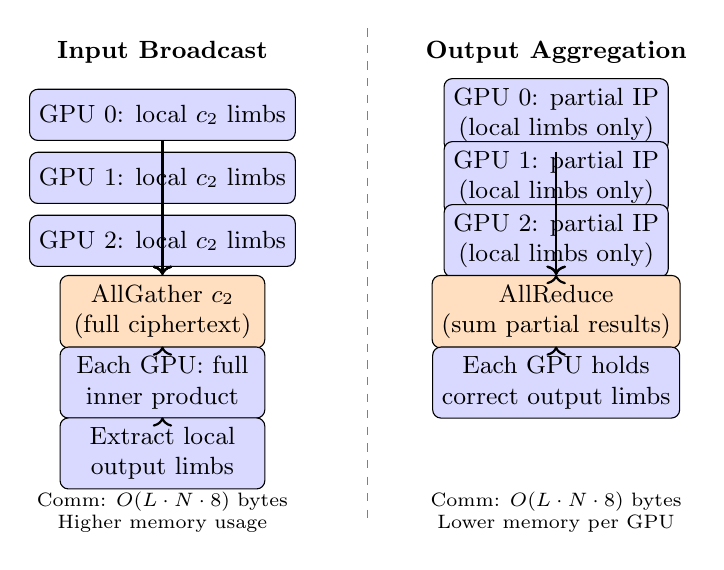
\begin{tikzpicture}[
  box/.style={draw, rounded corners=3pt, minimum width=2.6cm, minimum height=0.65cm,
              font=\small, align=center},
  comm/.style={box, fill=orange!25},
  compute/.style={box, fill=blue!15},
  arrow/.style={->, thick},
  gpu/.style={font=\footnotesize\bfseries}
]
  %--- Left: Input Broadcast ---
  \node[font=\small\bfseries] at (1.5, 4.0) {Input Broadcast};

  \node[compute] (g0a) at (1.5, 3.2) {GPU 0: local $c_2$ limbs};
  \node[compute] (g1a) at (1.5, 2.4) {GPU 1: local $c_2$ limbs};
  \node[compute] (g2a) at (1.5, 1.6) {GPU 2: local $c_2$ limbs};

  \node[comm]    (ag)  at (1.5, 0.7) {AllGather $c_2$\\(full ciphertext)};
  \draw[arrow] (g0a) -- (ag);
  \draw[arrow] (g1a) -- (ag);
  \draw[arrow] (g2a) -- (ag);

  \node[compute] (ip) at (1.5, -0.2) {Each GPU: full\\inner product};
  \draw[arrow] (ag) -- (ip);

  \node[compute] (ex) at (1.5, -1.1) {Extract local\\output limbs};
  \draw[arrow] (ip) -- (ex);

  \node[font=\scriptsize, align=center] at (1.5, -1.85)
    {Comm: $O(L \cdot N \cdot 8)$ bytes\\Higher memory usage};

  %--- Right: Output Aggregation ---
  \node[font=\small\bfseries] at (6.5, 4.0) {Output Aggregation};

  \node[compute] (g0b) at (6.5, 3.2) {GPU 0: partial IP\\(local limbs only)};
  \node[compute] (g1b) at (6.5, 2.4) {GPU 1: partial IP\\(local limbs only)};
  \node[compute] (g2b) at (6.5, 1.6) {GPU 2: partial IP\\(local limbs only)};

  \node[comm]    (ar)  at (6.5, 0.7) {AllReduce\\(sum partial results)};
  \draw[arrow] (g0b) -- (ar);
  \draw[arrow] (g1b) -- (ar);
  \draw[arrow] (g2b) -- (ar);

  \node[compute] (out) at (6.5, -0.2) {Each GPU holds\\correct output limbs};
  \draw[arrow] (ar) -- (out);

  \node[font=\scriptsize, align=center] at (6.5, -1.85)
    {Comm: $O(L \cdot N \cdot 8)$ bytes\\Lower memory per GPU};

  % Divider
  \draw[dashed, gray] (4.1, 4.3) -- (4.1, -2.0);

\end{tikzpicture}
\caption{Two multi-GPU key-switching algorithms. \textbf{Left (Input Broadcast):} each GPU
broadcasts its $c_2$ limbs so every GPU has the full $c_2$; then each GPU independently
computes the full inner product and keeps only its output limbs. \textbf{Right (Output
Aggregation):} each GPU computes a partial inner product from only its local limbs, then
AllReduce sums the partial results. Both transfer the same total data volume; Input Broadcast
uses more GPU memory but may overlap better with computation.}
\label{fig:keyswitch}
\end{figure}

% ---------------------------------------------------------------
% Figure: Multi-GPU swim-lane (Input Broadcast key-switch)
% ---------------------------------------------------------------
\begin{figure}[p]
\centering
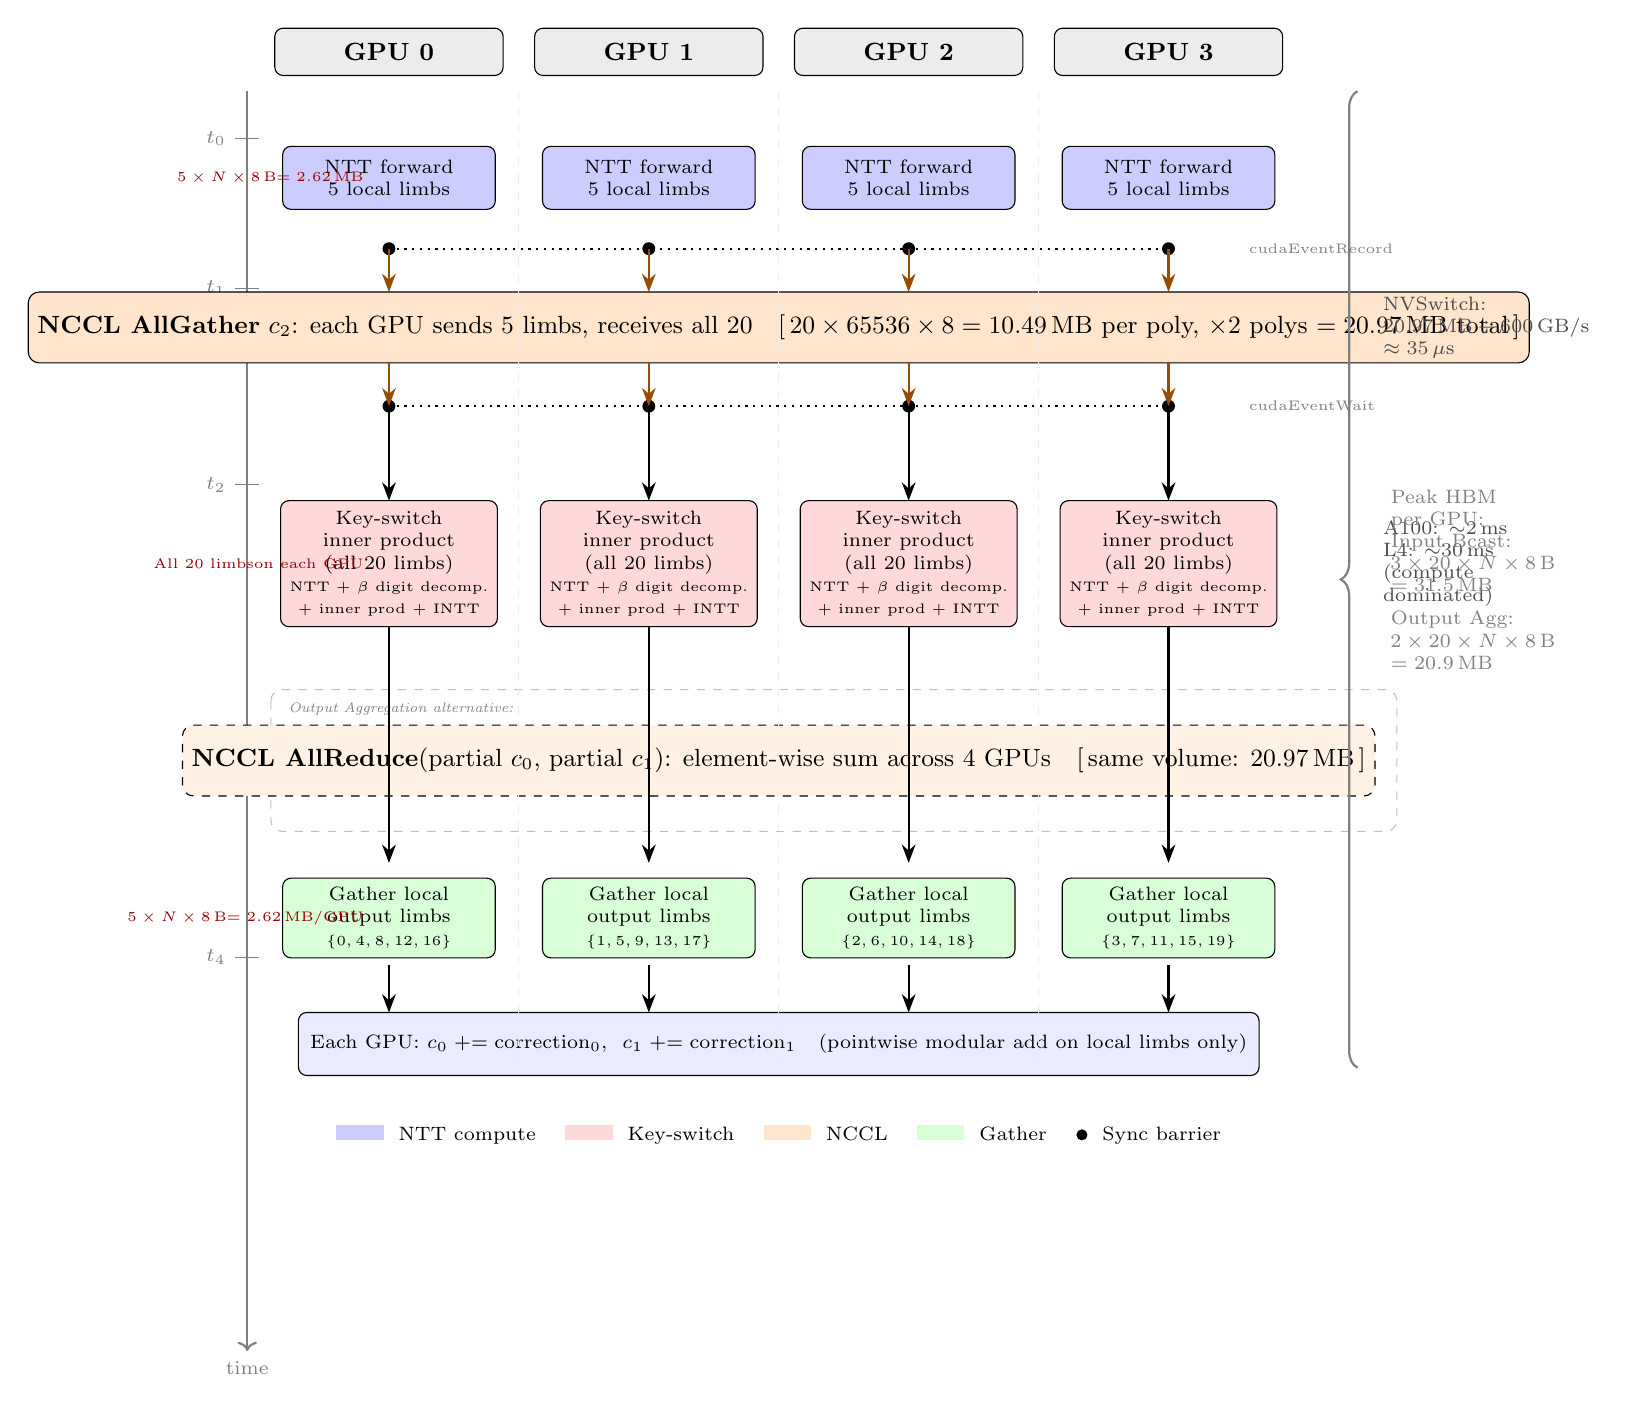
\begin{tikzpicture}[
  gpuhead/.style={draw, rounded corners=3pt, fill=gray!15,
                  minimum width=2.9cm, minimum height=0.6cm,
                  font=\small\bfseries, align=center},
  kblock/.style={draw, rounded corners=3pt, minimum width=2.7cm,
                 minimum height=0.8cm, font=\scriptsize,
                 align=center},
  ntt/.style   ={kblock, fill=blue!20},
  ks/.style    ={kblock, fill=red!15, minimum height=1.6cm},
  gather/.style={kblock, fill=green!15},
  ncclbar/.style={draw, fill=orange!20, rounded corners=4pt,
                  minimum height=0.9cm, font=\small, align=center},
  arr/.style={->, >=Stealth, thick},
  ann/.style={font=\scriptsize, gray!60!black, align=left,
              anchor=west},
  timeax/.style={font=\scriptsize, gray},
  datasz/.style={font=\tiny, red!60!black},
  sync/.style={draw, fill=black, circle, inner sep=1.5pt},
]

  % === Column positions ===
  \def\gA{0}    \def\gB{3.3}  \def\gC{6.6}  \def\gD{9.9}
  \def\mid{4.95}

  % === GPU headers ===
  \node[gpuhead] at (\gA, 0) {GPU 0};
  \node[gpuhead] at (\gB, 0) {GPU 1};
  \node[gpuhead] at (\gC, 0) {GPU 2};
  \node[gpuhead] at (\gD, 0) {GPU 3};

  % === Time axis (left) ===
  \draw[timeax, ->, thick] (-1.8, -0.5) -- (-1.8, -16.5)
    node[below, font=\scriptsize] {time};
  \foreach \y/\lab in {%
    -1.1/$t_0$, -3.0/$t_1$, -5.5/$t_2$,
    -9.0/$t_3$, -11.5/$t_4$} {
    \draw[timeax] (-1.95, \y) -- (-1.65, \y)
      node[left, font=\scriptsize] at (-1.95, \y) {\lab};
  }

  % === Phase 1: NTT on local limbs ===
  \node[ntt] (n0) at (\gA, -1.6) {NTT forward\\5 local limbs};
  \node[ntt] (n1) at (\gB, -1.6) {NTT forward\\5 local limbs};
  \node[ntt] (n2) at (\gC, -1.6) {NTT forward\\5 local limbs};
  \node[ntt] (n3) at (\gD, -1.6) {NTT forward\\5 local limbs};

  % Data size annotation
  \node[datasz, anchor=east] at (-0.2, -1.6)
    {$5 \times N \times 8$\,B\\$= 2.62$\,MB};

  % Sync barrier before NCCL
  \foreach \x in {\gA, \gB, \gC, \gD} {
    \node[sync] at (\x, -2.5) {};
  }
  \draw[dotted, thick] (\gA, -2.5) -- (\gD, -2.5);
  \node[font=\tiny, gray, anchor=west] at (10.8, -2.5)
    {cudaEventRecord};

  % === Phase 2: NCCL AllGather ===
  \node[ncclbar, minimum width=12.2cm] (ag) at (\mid, -3.5) {%
    \textbf{NCCL AllGather} $c_2$: each GPU sends 5 limbs,
      receives all 20\quad
    [\,$20 \times 65536 \times 8 = 10.49$\,MB per poly,
      $\times 2$ polys $= 20.97$\,MB total\,]%
  };
  \node[ann] at (12.5, -3.5) {NVSwitch:\\
    $20.97\,\text{MB} \div 600\,\text{GB/s}$\\$\approx 35\,\mu$s};

  % Sync barrier after NCCL
  \foreach \x in {\gA, \gB, \gC, \gD} {
    \node[sync] at (\x, -4.5) {};
  }
  \draw[dotted, thick] (\gA, -4.5) -- (\gD, -4.5);
  \node[font=\tiny, gray, anchor=west] at (10.8, -4.5)
    {cudaEventWait};

  % Connect NTT to AllGather
  \foreach \x in {\gA, \gB, \gC, \gD} {
    \draw[arr, orange!60!black] (\x, -2.5) -- (\x, -3.05);
    \draw[arr, orange!60!black] (\x, -3.95) -- (\x, -4.5);
  }

  % === Phase 3: Key-switch inner product (full c2) ===
  \node[ks] (k0) at (\gA, -6.5) {Key-switch\\inner product\\
    (all 20 limbs)\\
    {\tiny NTT + $\beta$ digit decomp.}\\
    {\tiny + inner prod + INTT}};
  \node[ks] (k1) at (\gB, -6.5) {Key-switch\\inner product\\
    (all 20 limbs)\\
    {\tiny NTT + $\beta$ digit decomp.}\\
    {\tiny + inner prod + INTT}};
  \node[ks] (k2) at (\gC, -6.5) {Key-switch\\inner product\\
    (all 20 limbs)\\
    {\tiny NTT + $\beta$ digit decomp.}\\
    {\tiny + inner prod + INTT}};
  \node[ks] (k3) at (\gD, -6.5) {Key-switch\\inner product\\
    (all 20 limbs)\\
    {\tiny NTT + $\beta$ digit decomp.}\\
    {\tiny + inner prod + INTT}};

  % Data size and timing
  \node[datasz, anchor=east] at (-0.2, -6.5)
    {All 20 limbs\\on each GPU};
  \node[ann] at (12.5, -6.5) {A100: ${\sim}$2\,ms\\
    L4: ${\sim}$30\,ms\\
    (compute\\dominated)};

  % Connect
  \foreach \x in {\gA, \gB, \gC, \gD} {
    \draw[arr] (\x, -4.5) -- (\x, -5.7);
  }

  % === Phase 4: AllReduce c0/c1 corrections (Output Agg path) ===
  % (show as optional alternative)
  \draw[dashed, gray!50, rounded corners=4pt]
    (-1.5, -8.1) rectangle (12.8, -9.9);
  \node[font=\tiny\itshape, gray, anchor=north west] at (-1.4, -8.15)
    {Output Aggregation alternative:};
  \node[ncclbar, minimum width=12.2cm, dashed,
        fill=orange!10] (ar) at (\mid, -9.0) {%
    \textbf{NCCL AllReduce}(partial $c_0$, partial $c_1$):
      element-wise sum across 4 GPUs\quad
    [\,same volume: 20.97\,MB\,]%
  };

  % === Phase 5: Extract local output limbs ===
  \node[gather] (g0) at (\gA, -11.0) {Gather local\\
    output limbs\\
    {\tiny $\{0,4,8,12,16\}$}};
  \node[gather] (g1) at (\gB, -11.0) {Gather local\\
    output limbs\\
    {\tiny $\{1,5,9,13,17\}$}};
  \node[gather] (g2) at (\gC, -11.0) {Gather local\\
    output limbs\\
    {\tiny $\{2,6,10,14,18\}$}};
  \node[gather] (g3) at (\gD, -11.0) {Gather local\\
    output limbs\\
    {\tiny $\{3,7,11,15,19\}$}};

  \node[datasz, anchor=east] at (-0.2, -11.0)
    {$5 \times N \times 8$\,B\\$= 2.62$\,MB/GPU};

  % Connect KS to gather
  \foreach \x in {\gA, \gB, \gC, \gD} {
    \draw[arr] (\x, -7.3) -- (\x, -10.3);
  }

  % === Phase 6: Result — apply corrections ===
  \node[kblock, fill=blue!8, minimum width=12.2cm] (done)
    at (\mid, -12.6) {%
    Each GPU: $c_0 \mathrel{+}= \text{correction}_0$,\ \
    $c_1 \mathrel{+}= \text{correction}_1$\quad
    (pointwise modular add on local limbs only)%
  };

  % Connect gather to done
  \foreach \x in {\gA, \gB, \gC, \gD} {
    \draw[arr] (\x, -11.6) -- (\x, -12.2);
  }

  % === Memory annotation (right side) ===
  \draw[decorate, decoration={brace, amplitude=6pt, mirror},
        thick, gray]
    (12.3, -0.5) -- (12.3, -12.9);
  \node[font=\scriptsize, gray, text width=2.2cm, align=left,
        anchor=west]
    at (12.6, -6.7) {Peak HBM\\per GPU:\\
    Input Bcast:\\
    $3 \times 20 \times N \times 8$\,B\\
    $= 31.5$\,MB\\[4pt]
    Output Agg:\\
    $2 \times 20 \times N \times 8$\,B\\
    $= 20.9$\,MB};

  % === Column dividers ===
  \foreach \x in {1.65, 4.95, 8.25} {
    \draw[gray!15, dashed] (\x, -0.5) -- (\x, -12.9);
  }

  % === Legend ===
  \node[font=\scriptsize, anchor=north, align=left] at (\mid, -13.5) {%
    \tikz\fill[blue!20] (0,0) rectangle (0.6,0.2); \ NTT compute
    \quad
    \tikz\fill[red!15] (0,0) rectangle (0.6,0.2); \ Key-switch
    \quad
    \tikz\fill[orange!20] (0,0) rectangle (0.6,0.2); \ NCCL
    \quad
    \tikz\fill[green!15] (0,0) rectangle (0.6,0.2); \ Gather
    \quad
    \tikz\fill[black] (0,0.07) circle (2pt); \ Sync barrier%
  };

\end{tikzpicture}
\caption{Multi-GPU swim-lane diagram for one key-switch operation
  (Input Broadcast algorithm, $n_\text{gpus}{=}4$, $L{=}20$ RNS
  limbs, $N{=}65536$).
  Each column is one GPU.
  Black dots mark CUDA event synchronization barriers.
  Phase~1: each GPU performs NTT on its 5~local limbs independently
  (no communication).
  Phase~2: NCCL AllGather broadcasts all limbs to every GPU
  (20.97\,MB, ${\sim}35\,\mu$s on NVSwitch).
  Phase~3: each GPU independently computes the full key-switch inner
  product over all 20~limbs (the compute bottleneck at ${\sim}2$\,ms
  on A100).
  Phase~4 (dashed): Output Aggregation alternative uses AllReduce
  instead, trading lower memory for a post-compute collective.
  Phase~5: each GPU extracts only its assigned output limbs (cyclic
  assignment).
  The right brace shows peak GPU HBM usage for each algorithm.
  On NVSwitch, communication is $<$2\% of compute time.}
\label{fig:ks-swimlane}
\end{figure}

\subsection{Concrete Communication Numbers}

For the GELU benchmark ($N=65536$, $L=20$, 8 GPUs on p4d.24xlarge NVSwitch at 600 GB/s):

\begin{itemize}
  \item AllGather volume per key-switch: $20 \times 65536 \times 8 \times 2 = 20.97\ \text{MB}$
  \item Time at 600 GB/s: $20.97\ \text{MB} \div 600\ \text{GB/s} \approx 35\ \mu\text{s}$
  \item Key-switch compute time on A100: $\sim 2\ \text{ms}$
  \item \textbf{Communication overhead: $\sim 1.7\%$ of compute} --- nearly free on NVSwitch
\end{itemize}

On MareNostrum 5 InfiniBand (25 GB/s effective inter-node):
\begin{itemize}
  \item Time for same AllGather: $\approx 840\ \mu\text{s}$
  \item Communication overhead: $\sim 42\%$ of compute --- significant; overlap is critical
\end{itemize}

\subsection{CUDA Streams and Overlap}

Each GPU runs computation and communication concurrently using multiple CUDA streams.
Figure~\ref{fig:overlap} shows the overlap strategy.

\begin{figure}[ht!]
\centering
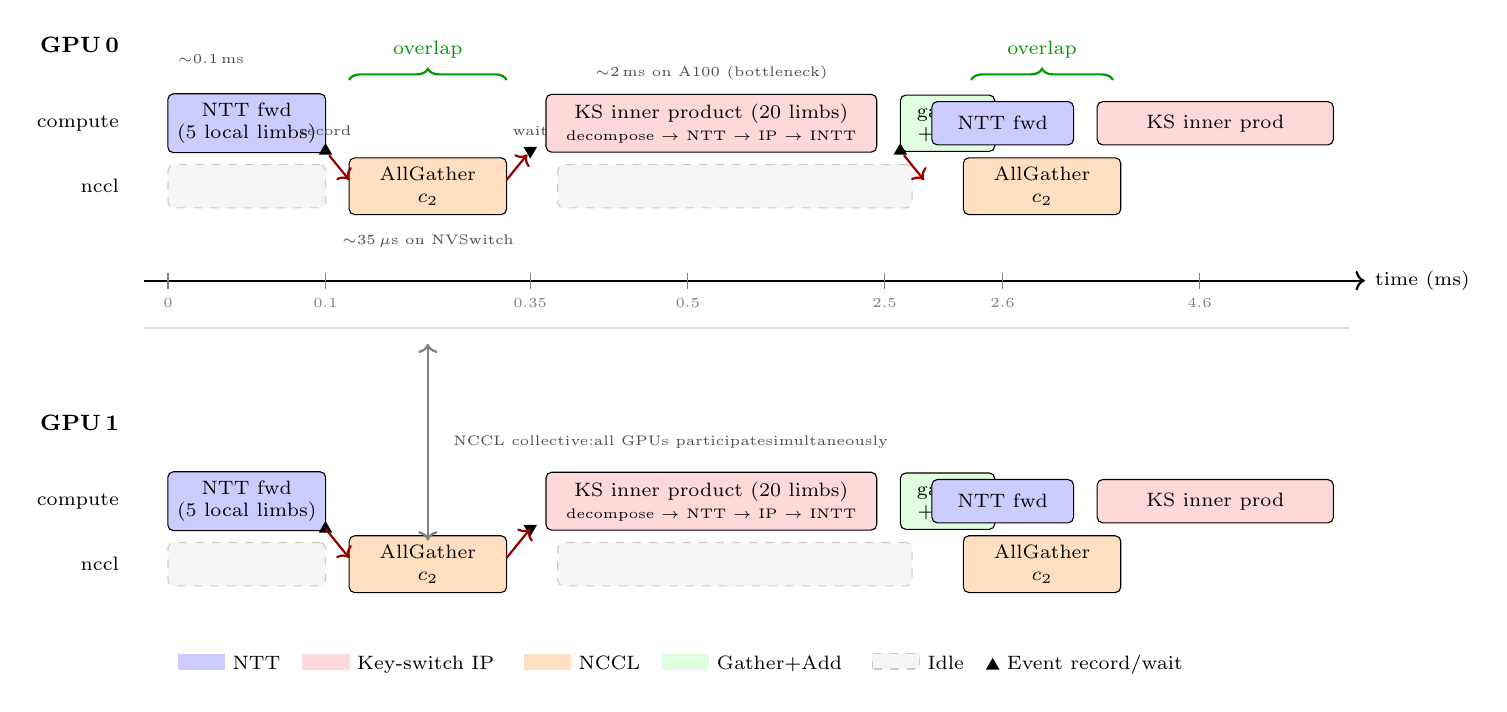
\begin{tikzpicture}[
  task/.style={draw, minimum height=0.55cm, font=\scriptsize,
               align=center, rounded corners=2pt},
  ntt/.style  ={task, fill=blue!20},
  ks/.style   ={task, fill=red!15},
  add/.style  ={task, fill=green!12},
  nccl/.style ={task, fill=orange!25},
  idle/.style ={task, fill=gray!8, dashed, draw=gray!40},
  evrecord/.style={fill=black, regular polygon,
    regular polygon sides=3, inner sep=1pt,
    font=\tiny},
  evwait/.style={fill=black, regular polygon,
    regular polygon sides=3, inner sep=1pt,
    rotate=180, font=\tiny},
  ann/.style={font=\tiny, gray!60!black},
]

  % === Time axis ===
  \draw[->, thick] (-0.3, -1.2) -- (15.2, -1.2)
    node[right, font=\scriptsize] {time (ms)};
  \foreach \x/\t in {0/0, 2/0.1, 4.6/0.35, 6.6/0.5, 9.1/2.5,
                     10.6/2.6, 13.1/4.6} {
    \draw[gray] (\x, -1.3) -- (\x, -1.1);
    \node[font=\tiny, gray, below] at (\x, -1.3) {\t};
  }

  % === Row labels ===
  \node[anchor=east, font=\footnotesize\bfseries] at (-0.5, 1.8)
    {GPU\,0};
  \node[anchor=east, font=\scriptsize] at (-0.5, 0.8)
    {compute};
  \node[anchor=east, font=\scriptsize] at (-0.5, 0.0)
    {nccl};

  \node[anchor=east, font=\footnotesize\bfseries] at (-0.5, -3.0)
    {GPU\,1};
  \node[anchor=east, font=\scriptsize] at (-0.5, -4.0)
    {compute};
  \node[anchor=east, font=\scriptsize] at (-0.5, -4.8)
    {nccl};

  % Horizontal separator
  \draw[gray!30] (-0.3, -1.8) -- (15.0, -1.8);

  % ============== GPU 0 ==============

  % --- Key-switch operation A ---
  % Compute stream
  \node[ntt, minimum width=2.0cm]  (g0nttA) at (1.0, 0.8)
    {NTT fwd\\(5 local limbs)};
  \node[ks,  minimum width=4.2cm]  (g0ksA)  at (6.9, 0.8)
    {KS inner product (20 limbs)\\
     {\tiny decompose $\to$ NTT $\to$ IP $\to$ INTT}};
  \node[add, minimum width=1.2cm]  (g0addA) at (9.9, 0.8)
    {gather\\+ add};

  % NCCL stream
  \node[idle, minimum width=2.0cm] at (1.0, 0.0) {};
  \node[nccl, minimum width=2.0cm] (g0agA) at (3.3, 0.0)
    {AllGather\\$c_2$};
  \node[idle, minimum width=4.5cm] at (7.2, 0.0) {};

  % --- Key-switch operation B (pipelined) ---
  \node[ntt, minimum width=1.8cm]  (g0nttB) at (10.6, 0.8)
    {NTT fwd};
  \node[ks,  minimum width=3.0cm]  (g0ksB)  at (13.3, 0.8)
    {KS inner prod};
  \node[nccl, minimum width=2.0cm] (g0agB) at (11.1, 0.0)
    {AllGather\\$c_2$};

  % Event markers GPU 0
  \node[evrecord] (e0r1) at (2.0, 0.45) {};
  \node[ann, anchor=south] at (2.0, 0.52) {record};
  \draw[->, thick, red!60!black] (e0r1) -- (2.3, 0.08);

  \node[evwait] (e0w1) at (4.6, 0.45) {};
  \node[ann, anchor=south] at (4.6, 0.52) {wait};
  \draw[->, thick, red!60!black] (4.3, 0.08) -- (e0w1);

  \node[evrecord] (e0r2) at (9.3, 0.45) {};
  \draw[->, thick, red!60!black] (e0r2) -- (9.6, 0.08);

  % Overlap brace A
  \draw[decorate, decoration={brace, amplitude=4pt},
        green!60!black, thick]
    (2.3, 1.35) -- (4.3, 1.35)
    node[midway, above=4pt, font=\scriptsize, green!60!black]
      {overlap};

  % Overlap brace B
  \draw[decorate, decoration={brace, amplitude=4pt},
        green!60!black, thick]
    (10.2, 1.35) -- (12.0, 1.35)
    node[midway, above=4pt, font=\scriptsize, green!60!black]
      {overlap};

  % ============== GPU 1 (identical, offset) ==============

  % Compute stream
  \node[ntt, minimum width=2.0cm]  at (1.0, -4.0)
    {NTT fwd\\(5 local limbs)};
  \node[ks,  minimum width=4.2cm]  at (6.9, -4.0)
    {KS inner product (20 limbs)\\
     {\tiny decompose $\to$ NTT $\to$ IP $\to$ INTT}};
  \node[add, minimum width=1.2cm]  at (9.9, -4.0)
    {gather\\+ add};
  \node[ntt, minimum width=1.8cm]  at (10.6, -4.0)
    {NTT fwd};
  \node[ks,  minimum width=3.0cm]  at (13.3, -4.0)
    {KS inner prod};

  % NCCL stream
  \node[idle, minimum width=2.0cm] at (1.0, -4.8) {};
  \node[nccl, minimum width=2.0cm] at (3.3, -4.8)
    {AllGather\\$c_2$};
  \node[idle, minimum width=4.5cm] at (7.2, -4.8) {};
  \node[nccl, minimum width=2.0cm] at (11.1, -4.8)
    {AllGather\\$c_2$};

  % Event markers GPU 1
  \node[evrecord] at (2.0, -4.35) {};
  \draw[->, thick, red!60!black] (2.0, -4.35) -- (2.3, -4.72);
  \node[evwait]   at (4.6, -4.35) {};
  \draw[->, thick, red!60!black] (4.3, -4.72) -- (4.6, -4.35);

  % === Annotations ===
  % Timing callouts
  \node[ann, anchor=north west] at (0, 1.8)
    {${\sim}0.1$\,ms};
  \node[ann, anchor=north] at (3.3, -0.5)
    {${\sim}35\,\mu$s on NVSwitch};
  \node[ann, anchor=north] at (6.9, 1.65)
    {${\sim}2$\,ms on A100 (bottleneck)};

  % NCCL sync label
  \draw[<->, gray, thick] (3.3, -2.0) -- (3.3, -4.5);
  \node[ann, anchor=west] at (3.5, -3.25)
    {NCCL collective:\\all GPUs participate\\simultaneously};

  % === Legend ===
  \node[font=\scriptsize, anchor=north west] at (0, -5.8) {%
    \tikz\fill[blue!20]   (0,0) rectangle (0.6,0.2);\ NTT\quad
    \tikz\fill[red!15]    (0,0) rectangle (0.6,0.2);\ Key-switch IP
      \quad
    \tikz\fill[orange!25] (0,0) rectangle (0.6,0.2);\ NCCL\quad
    \tikz\fill[green!12]  (0,0) rectangle (0.6,0.2);\ Gather+Add
      \quad
    \tikz\fill[gray!8, draw=gray!40, dashed]
      (0,0) rectangle (0.6,0.2);\ Idle\quad
    \tikz\node[fill=black, regular polygon,
      regular polygon sides=3, inner sep=1pt]{};\ Event
      record/wait%
  };

\end{tikzpicture}
\caption{Compute-communication overlap Gantt chart for two consecutive
  key-switch operations on two GPUs.
  Each GPU has two CUDA streams: \textit{compute} (NTT, key-switch
  inner product, gather) and \textit{nccl} (AllGather/AllReduce
  collectives).
  Black triangles mark \texttt{cudaEventRecord} (on compute stream)
  and \texttt{cudaEventWait} (before compute reads NCCL output);
  red arrows show the dependency direction.
  Green braces highlight where NCCL communication runs concurrently
  with compute---on NVSwitch, the 35\,$\mu$s AllGather is fully hidden
  behind the $\sim$2\,ms inner product, giving $<$2\% communication
  overhead.
  The second key-switch (operation~B) begins its AllGather while
  operation~A's gather+add completes, demonstrating pipeline
  parallelism across successive operations.}
\label{fig:overlap}
\end{figure}

Each GPU maintains:
\begin{itemize}
  \item \textbf{Compute stream}: NTT, polynomial arithmetic, inner product,
    gather/scatter kernels
  \item \textbf{NCCL stream}: AllGather and AllReduce collectives
  \item \textbf{CUDA events}: \texttt{compute\_done} (signaling NTT
    complete, safe to issue NCCL) and \texttt{nccl\_done} (signaling
    collective complete, safe to read received data)
\end{itemize}

CUDA events synchronize the two streams at the dependency boundary: the compute stream
records an event after NTT completes, the NCCL stream waits on it before issuing the
collective; conversely, the compute stream waits on the NCCL event before starting the
inner product that reads communicated data.
An optional \textbf{CudaGraph capture} of the full bootstrapping pipeline eliminates the
$\sim 250\ \mu\text{s}$ kernel launch overhead for the many sequential operations in
StoC/CtoS.

%============================================================
\section{Source Code: Multi-GPU Implementation Files}
\label{sec:srcfiles}
%============================================================

\subsection{Directory: \texttt{src/multi\_gpu/}}

\begin{description}
  \item[\texttt{comm/nccl\_comm.cuh/.cu}] NCCL wrapper for ciphertext collectives:
    \texttt{broadcast\_rns\_limb()}, \texttt{allgather\_ct()}, \texttt{allreduce\_partial()}.
    Contains \texttt{MultiGpuContext} (holds NCCL communicators + CUDA streams for all GPUs)
    and \texttt{LimbRange} (describes which limbs a GPU owns).
  \item[\texttt{partition/rns\_partition.cuh/.cu}] RNS limb-to-GPU assignment:
    \texttt{owner\_of\_limb(j, n\_gpus)}, \texttt{local\_index\_of\_limb()}, \texttt{n\_local\_limbs()}.
    CUDA kernels \texttt{kernel\_scatter\_limbs()} and \texttt{kernel\_gather\_limbs()} for
    GPU-side scatter/gather without CPU involvement.
  \item[\texttt{keyswitching/input\_broadcast.cuh/.cu}] Input Broadcast key-switching:
    each GPU broadcasts its $c_2$ limbs via AllGather; all GPUs compute full inner product.
  \item[\texttt{keyswitching/output\_aggregation.cuh/.cu}] Output Aggregation key-switching:
    each GPU computes partial inner product from local limbs; AllReduce merges results.
  \item[\texttt{overlap/stream\_manager.cuh/.cu}] CUDA stream pool, event synchronization,
    \texttt{OverlapScheduler} for compute--communication overlap, optional CudaGraph capture.
  \item[\texttt{nvtx\_ranges.cuh}] NVIDIA NVTX annotations marking key operations for
    Nsight Systems timeline visualization.
\end{description}

\subsection{Directory: \texttt{src/benchmarks/}}

\begin{description}
  \item[\texttt{nccl\_bandwidth\_test.cu}] Validates NCCL setup; measures NVSwitch/InfiniBand
    bandwidth for AllGather, AllReduce, Broadcast at ciphertext-sized messages.
  \item[\texttt{bert\_inference.cu}] End-to-end BERT-base benchmark: runs NEXUS inference
    pipeline with \texttt{--n-gpus 1/2/4/8}; outputs per-layer breakdown CSV with columns
    \texttt{n\_gpus, total\_ms, keyswitch\_ms, comm\_ms, speedup, efficiency}.
  \item[\texttt{bootstrapping\_bench.cu}] Isolated bootstrapping benchmark: measures
    bootstrapping latency vs.\ number of GPUs; reports mean/min/max/stddev over iterations.
\end{description}

%============================================================
\section{Build System}
\label{sec:build}
%============================================================

\begin{lstlisting}[style=bash, caption=Building on AWS g4dn.2xlarge (T4 GPU)]
# Environment setup (sets CUDA, NCCL, MPI paths)
source scripts/aws/setup_p4d_env.sh

# Build all targets (sm_75 for T4; use sm_80 for A100, sm_90 for H100)
mkdir build && cd build
cmake .. -DCMAKE_CUDA_ARCHITECTURES=75
make -j8

# Run single-GPU NEXUS baseline
./benchmarks/nexus_bert_baseline

# Run multi-GPU BERT inference (once multi-GPU quota approved)
./benchmarks/bert_inference --n-gpus 1
\end{lstlisting}

The CMakeLists.txt in the project root:
\begin{itemize}
  \item Requires: CUDA 12.x, NCCL 2.x, MPI (for multi-node)
  \item Finds Phantom as a subdirectory (via \texttt{add\_subdirectory})
  \item GLOB collects \texttt{.cu} files from \texttt{src/multi\_gpu/} into a static library
  \item Each benchmark is an executable linking against the static library + Phantom + NCCL
  \item GPU architectures: 75 (T4), 80 (A100), 90 (H100) --- set with \texttt{-DCMAKE\_CUDA\_ARCHITECTURES}
\end{itemize}

%============================================================
\section{Profiling Guide}
\label{sec:profiling}
%============================================================

\subsection{Tools Required}

\begin{description}
  \item[Nsight Systems (\texttt{nsys})] System-level timeline profiler. Shows CPU--GPU
    synchronization, NCCL collectives, kernel launch overhead, memory transfers. Runs
    across the full application.
  \item[Nsight Compute (\texttt{ncu})] Kernel-level profiler. Measures roofline
    metrics: compute throughput (TFLOP/s), memory bandwidth (GB/s), occupancy, warp
    stalls for individual CUDA kernels.
\end{description}

\subsection{Step-by-Step Profiling on EC2}

\begin{lstlisting}[style=bash, caption=System profiling with Nsight Systems]
# Profile full BERT inference, generate timeline
bash profiling/nsys_profile.sh ./benchmarks/bert_inference --n-gpus 1

# Output: bert_profile.nsys-rep
# Open in Nsight Systems GUI (locally via X11 forwarding or SSH tunnel)
nsys-ui bert_profile.nsys-rep
\end{lstlisting}

\begin{lstlisting}[style=bash, caption=Kernel profiling with Nsight Compute (NTT focus)]
# Profile only the NTT kernel for roofline analysis
bash profiling/ncu_ntt_profile.sh ./benchmarks/bert_inference --n-gpus 1

# Key metrics to collect:
# - sm__throughput.avg.pct_of_peak_sustained_elapsed (compute utilization)
# - l1tex__t_bytes.sum / l2_global_load / dram_read_transactions (memory)
# - achieved_occupancy (warp occupancy vs. theoretical max)
# - stall_long_scoreboard (memory latency stalls)
\end{lstlisting}

\subsection{Metrics to Look For}

\begin{table}[h]
\centering
\begin{tabular}{@{}lll@{}}
\toprule
\textbf{Operation} & \textbf{Bottleneck Indicator} & \textbf{Target on A100} \\
\midrule
NTT forward/inverse & Memory bandwidth bound & $>80\%$ HBM bandwidth \\
Key-switch inner prod & Compute bound & $>50\%$ FP64 throughput \\
RNS modular reduction & Compute bound & High int64 throughput \\
NCCL AllGather & Network bound & $>400$ GB/s aggregate \\
Bootstrap CtoS/StoC & Mixed: rotation + multiply & Balanced \\
\bottomrule
\end{tabular}
\caption{Expected bottleneck profiles for each NEXUS operation on A100.}
\end{table}

\subsection{Identifying NTT, Key-Switch, and Bootstrapping Bottlenecks}

In the Nsight Systems timeline, look for:

\begin{itemize}
  \item \textbf{NTT}: Kernel names containing \texttt{nwt\_2d\_radix8}. Should be
    short and frequent. If they take $>50\%$ of total time, the NTT is the bottleneck.
  \item \textbf{Key-switching}: Kernel names containing \texttt{key\_switch\_inner\_prod}.
    Often the single most expensive kernel per FHE multiply.
  \item \textbf{Bootstrapping}: A cluster of $>30$ sequential operations (NTT +
    multiply-plain + rotate). Identifiable by the long uninterrupted GPU segment.
  \item \textbf{NCCL}: Colored segments labeled \texttt{ncclAllGather} or
    \texttt{ncclAllReduce}. On NVSwitch these should be very short; on InfiniBand they
    will be visible gaps.
\end{itemize}

\subsection{Expected Results and Plotting}

Expected speedup for BERT inference on p4d.24xlarge:

\begin{table}[h]
\centering
\begin{tabular}{@{}lrrr@{}}
\toprule
\textbf{GPUs} & \textbf{Expected Time (s)} & \textbf{Speedup} & \textbf{Efficiency} \\
\midrule
1 (A100) & 37.3 & 1.0$\times$ & 100\% \\
2 & $\sim$20 & 1.9$\times$ & 95\% \\
4 & $\sim$11 & 3.4$\times$ & 85\% \\
8 & $\sim$7 & 5.3$\times$ & 66\% \\
\bottomrule
\end{tabular}
\caption{Expected BERT-base inference latency scaling (based on Cerium results for similar FHE workloads).}
\end{table}

To generate scaling plots from result CSVs:

\begin{lstlisting}[style=bash, caption=Generating speedup plots]
# Run experiments (on EC2, once quota approved)
for gpus in 1 2 4 8; do
  ./benchmarks/bert_inference --n-gpus $gpus \
    --output experiments/results/YYYY-MM-DD_a100x${gpus}_scaling-bert/raw/bert_${gpus}gpu.csv
done

# Plot (locally)
python3 experiments/plot_scaling.py \
  --input experiments/results/ \
  --output experiments/plots/YYYY-MM-DD_bert_scaling.pdf
\end{lstlisting}

%============================================================
\section{Glossary}
%============================================================

\begin{description}
  \item[CKKS] Cheon-Kim-Kim-Song: an FHE scheme for approximate real-number arithmetic
  \item[RNS] Residue Number System: representing large integers as tuples modulo small primes
  \item[NTT] Number Theoretic Transform: modular-arithmetic FFT for fast polynomial multiplication
  \item[RLWE] Ring Learning With Errors: the computational hardness assumption underlying CKKS
  \item[Key-switching] Converting a ciphertext encrypted under one key to one encrypted under another; used for relinearization and rotation
  \item[Bootstrapping] A procedure to refresh a ciphertext's level budget, enabling unlimited computation depth
  \item[BSGS] Baby-Step Giant-Step: algorithmic trick to reduce rotation count from $O(N)$ to $O(\sqrt{N})$
  \item[NCCL] NVIDIA Collective Communications Library: optimized multi-GPU/multi-node collectives
  \item[Rescale] A CKKS-specific operation that divides ciphertext by one prime, reducing both level and scale
  \item[Chain index] The current level of a ciphertext in the modulus chain (0 = freshest, increases as levels are consumed)
  \item[Slot] One of the $N/2$ independent complex numbers that can be packed into one CKKS ciphertext
  \item[Galois key] A key enabling one specific rotation of the slot vector; one key per rotation step
  \item[Relin key] Relinearization key: used to reduce size-3 to size-2 after ciphertext multiplication
  \item[p4d.24xlarge] AWS EC2 instance with 8$\times$ A100 40 GB GPUs, NVSwitch interconnect, EFA networking
  \item[NVSwitch] NVIDIA's high-bandwidth GPU-to-GPU interconnect in A100 DGX nodes (600 GB/s per GPU)
  \item[MAE] Mean Absolute Error: metric for quantifying approximation error after FHE computation
  \item[Input Broadcast] Key-switching algorithm: AllGather $c_2$ so every GPU has the full polynomial, then local inner product
  \item[Output Aggregation] Key-switching algorithm: each GPU computes partial inner product, AllReduce merges results
  \item[CudaGraph] CUDA feature for capturing and replaying a sequence of kernels with near-zero launch overhead
\end{description}

%============================================================
\section{Next Steps and Current Status}
%============================================================

\subsection{Current Status (March 2026)}

\begin{itemize}
  \item All source code written (\texttt{src/multi\_gpu/}, \texttt{src/benchmarks/}) with correct API structure and TODO stubs at Phantom integration points.
  \item AWS quota for 96 vCPUs (p4d.24xlarge) has been requested and rejected due to no billing history.
  \item Immediate plan: run on \textbf{g4dn.2xlarge} (8 vCPU + 1$\times$ T4) to establish spending history and collect single-GPU baseline profiling data.
\end{itemize}

\subsection{g4dn.2xlarge Experiments (Immediate)}

\begin{enumerate}
  \item \textbf{Build}: compile with \texttt{-DCMAKE\_CUDA\_ARCHITECTURES=75} for T4 (CC 7.5).
  \item \textbf{Correctness}: run each NEXUS sub-benchmark (MatMul, GELU, SoftMax, LayerNorm, Argmax) and verify MAE matches reference values.
  \item \textbf{Baseline timing}: record T4 latency per operation; expect $\sim$3--5$\times$ slower than A100 due to lower HBM bandwidth (320 vs.\ 2000 GB/s).
  \item \textbf{Profiling}: run Nsight Systems to capture kernel-level timeline; identify what fraction of time is NTT vs.\ key-switching vs.\ bootstrapping.
  \item \textbf{Level tracing}: confirm the 31-level budget in Table~\ref{tab:levels}.
\end{enumerate}

\subsection{p4d.24xlarge Experiments (After Quota Approval)}

\begin{enumerate}
  \item Reproduce the NEXUS 37s baseline on A100 (\texttt{--n-gpus 1}).
  \item Run multi-GPU scaling sweep: 1, 2, 4, 8 GPUs; collect CSV results.
  \item Compare Input Broadcast vs.\ Output Aggregation key-switching algorithms.
  \item Run isolated bootstrapping benchmark to quantify BSGS rotation overhead.
  \item Generate scaling plots; compare against Table~\ref{tab:speedup} predictions.
\end{enumerate}

\subsection{Multi-Node (MareNostrum 5, Future)}

Once single-node multi-GPU is validated, the next step is inter-node experiments on
MareNostrum 5 (up to 16$\times$ H100 across 4 nodes). The InfiniBand communication
overhead becomes significant (see Table~\ref{tab:commtime}), and the CudaGraph and
compute-communication overlap machinery will be critical to achieving acceptable speedup.

\end{document}
